%snake surrounding stuff

%visual hull

%NASA cams

% Aikaisempi tutkimus
\section{Image acquisition}

% TODO: image of a scene, a camera and a computer, all connected

Digital stereo vision in the end analyses digital images for depth cues.
A digital photograph is variations in light on an image sensor that has been digitized.
In front of a sensor is a lens system that projects an image to the sensor.

This section describes the theory for basic image acquisition steps and main concerns that affect reconstruction quality.

%At first, the pipeline from a real-life scene to an image file on a computer is described.
%Then, the theory is extended to video, i.e. capturing motion as a sequence of images.
%Next, major properties of interest of commercial cameras are discussed. Finally, 

Reconstruction accuracy and errors depend on not only decidable physical parameters of a stereo imaging rig, such as camera positioning accuracy, but also on e.g. lens imperfections, camera focus, camera sensor noise, image compression and algorithmic accuracy. \cite{hollsten2013imagequality, kyto2011method,rieke2009evaluation}.

\subsection{Imaging} \label{sec:imaging} % {{{

Images are commonly taken with digital cameras that project a three-dimensional view from a single viewpoint to an image plane, and finally to a discrete grid of numerical values that describe light intensities.
%In addition to plain photographic cameras, reconstruction can be done using e.g. laser scanners or light field cameras. Those are not covered in this work.

% }}} imaging

\subsubsection{Pinhole camera} \label{sec:pinhole} % {{{

%near objects look bigger than distant objects

% What's a pinhole camera, what projection means.

\simplegfx{h}{0.6\textwidth}{pinhole-camera}
{Pinhole camera principle. The box represents a camera; image seen through the small hole is formed to the planar film or sensor on its back, rotated upside down, as rays of light go from the subject through the hole.}

A physical camera is in its simplest form modeled as a pinhole camera; an ideal device that projects an image upside down on its film through an infinitesimal aperture.
Illustration given in image \ref{fig:pinhole-camera}.
The term \emph{projection} is the representation of three-dimensional objects on a flat surface, seen from a single point such as the human eye.
A cube projected on a plane is shown in figure \ref{fig:perspproj}.

\simplegfx{h}{0.6\textwidth}{perspproj}
{Perspective projection: a cube seen from origin O projected on a plane; point P projects to p. In a camera, the rays of light travel through a common point to the film that is behind the origin; a virtual projection film between the origin and the object is often used for simplicity.}

% http://en.wikipedia.org/wiki/Perspective_projection rays of light etc.

% Cartesian coordinates.

Mathematically, a point in a three-dimensional world can be encoded in any coordinate system;
when using a cartesian coordinate system, a point is described as a location relative to a selected origin reference, as a triplet of distances along three perpendicular X, Y and Z axes (figure \ref{fig:coordsys}).
In a traditional right-handed system, X increases right, Y upwards and Z towards the viewer.
All coordinates throughout this work are expressed in a 3D cartesian system, unless noted otherwise.

\simplegfx{h}{0.6\textwidth}{coordsys}
{A 3D cartesian coordinate system. Origin at O, point location encoded in the triplet $(x,y,z)$ as individual lengths along the X, Y and Z axes, respectively.}

% Points, projection equation.

\subsubsection{Pinhole math that should go to next main section}

Light rays travel through the pinhole camera's aperture to the image plane that is $f$ units behind the aperture, while the camera origin is set to the aperture.
The pinhole model (or, perspective projection) states that the world point $(x, y, z)$ is projected to the 2D image plane at $(u, v)$:

\begin{equation}
\begin{pmatrix}
u \\ v
\end{pmatrix}
=
-\frac{f}{z} \begin{pmatrix}
x \\ y
\end{pmatrix}
\end{equation}

The result can be derived from similar triangles with a common vertex at the aperture; figure \ref{fig:pinhole3d}.

Sometimes the sign is inverted, which results in a plane on the other side of the origin where the actual point lies, where the image is not rotated; this can be more convenient to analyse.
\cite{hartley03multiview}

% Matrices, homogeneous coordinates.

% projective element, "~" up to scale equality definition

This projection is given as a $3 \times 4$ matrix, when 3D points are expressed in homogeneous coordinates.
Homogeneous coordinates add an extra dimension to the interpretation of coordinates, and each point becomes a line that crosses the origin in a dimension one higher than the original.
In addition, several vector operations become more convenient to manipulate; for example, 3D translation is embedded in 4D matrices with homogeneous coordinates. \cite{hartley03multiview,heyden2005multiple}

Setting the camera to origin and using homogeneous coordinates, the mapping is given with a camera matrix as

\begin{equation}
\begin{pmatrix}
u \\ v \\ 1
\end{pmatrix}
=
\begin{pmatrix}
xf/z \\ yf/z \\ 1
\end{pmatrix}
\sim
\begin{pmatrix}
x \\ y \\ z/f
\end{pmatrix}
=
\begin{pmatrix} \label{eq:cmat}
	1 & 0 & 0 & 0 \\
	0 & 1 & 0 & 0 \\
	0 & 0 & 1/f & 0
\end{pmatrix}
\begin{pmatrix}
x \\ y \\ z \\ 1
\end{pmatrix}
\end{equation}

The camera position and rotation in a global coordinate frame can be encoded in a matrix so that the point $(x,y,z)$ in global coordinate frame is first transformed from a global coordinate frame to a camera-centered frame; section \ref{sec:coord} discusses this in more detail.

% }}} pinhole

\subsubsection{Optics} % {{{

%Practical algorithms take lens imperfections into account (e.g. \cite{opencv}).

In practice, no actual camera works ideally; a pinhole-resembling camera could be built, but it would have poor light gathering power and low resolution limited by diffraction effects. \cite{todo}
Imperfections in the lenses project points to positions that differ from those predicted by straight lines in this linear case.
Lens distortions deviate the rays, and no system is in perfect focus, so that one point spreads out as a circle.
%In reconstructing, methods that estimate the points and minimize errors are used, as no model predicts the camera perfectly.

Construction of optical systems is well studied. \cite{kingslake1989history}
Actual camera ``lenses'' consist of not only a single glass element (optical lens) but many, especially in the case of zoom lenses whose focal length can be changed.
As an example, a Canon lens diagram is shown in figure \ref{fig:canonef50mm}.
There are several lenses, some grouped together, all aligned so that their centers lie parallel to the optical axis.
Optical stabilization in a camera lens is implemented with a moving element in the middle of the lens.
%In this work, the inner workings of these systems are ignored and equations assume a simple projective model, which is a safe assumption when the image is in focus.

% http://www.canon.com/camera-museum/lens/ef/data/standard/ef_50_18ii.html?p=2
%\simplegfx{h!}{0.6\textwidth}{canonef50mm}
%{Block diagram of Canon EF50mm f/1.8 II lens construction; insides of the lens shown from the side.}

\simplefig{h}{%
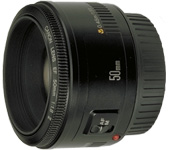
\includegraphics[width=0.4\textwidth]{gfx/canonef50mm-1}
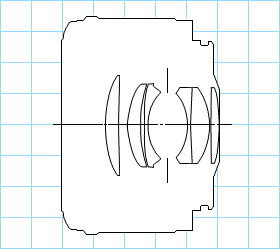
\includegraphics[width=0.4\textwidth]{gfx/canonef50mm-2}
}{fig:canonef50mm}
{A fixed focal length Canon EF 50mm f/1.8 II lens. Left: the lens. Right: block diagram of the lens construction, showing the six optical elements. Diagram by Canon Camera Museum.}


The following equation applies for a thin lens and image in focus, illustrated in figure \ref{fig:thinlens}:

\begin{equation}
	\frac{1}{a} + \frac{1}{b} = \frac{1}{f} \label{eq:focal}
\end{equation}

\simplefig{h!}{\documentclass{standalone}
\usepackage{tikz}
\begin{document}

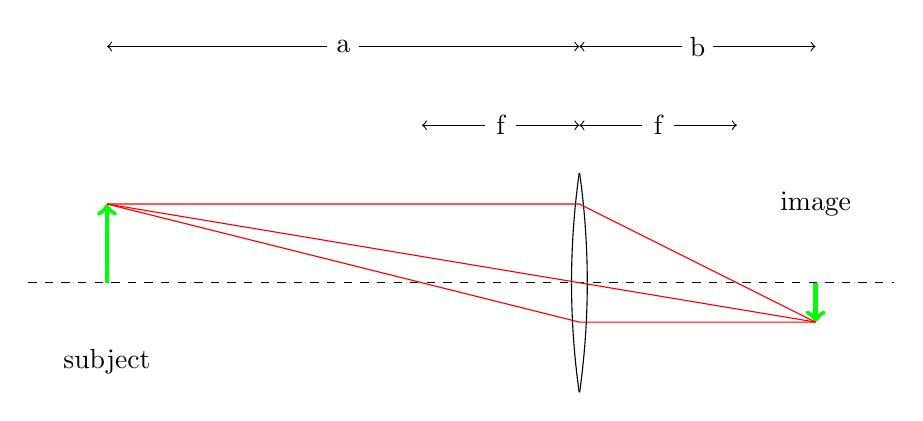
\begin{tikzpicture}

%\namedhorline{text}{textpos}{radius}
\newcommand*{\namedhorline}[3]{%
	%\draw [<-] ++ -- ++(\dx,\dy) -- ++(\dx,-\dy) -- ++(-\dx,-\dy) -- cycle
	\draw [->] (#2) +(-0.2,0) -- +(-#3,0);
	\node at (#2) {#1};
	\draw [->] (#2) +(0.2,0) -- +(#3,0);
}

\def\rad{10}
\def\ang{8}

\def\lensx{0}
\def\lensy{0}
\def\lensw{0.2}

\def\objh{1}
\def\imgh{0.5}
\def\objx{6}
\def\imgx{3}
\def\f{2}
% 1/3 + 1/6 = 1/2

\def\flabely{2}
\def\alabely{3}

% background
\draw [dashed] (-\objx-1, 0) -- (\imgx+1, 0);

% lens

\draw (\lensx+\lensw/2,\lensy) arc [radius=\rad, start angle=0, end angle=\ang];
\draw (\lensx+\lensw/2,\lensy) arc [radius=\rad, start angle=0, end angle=-\ang];

\draw (\lensx-\lensw/2,\lensy) arc [radius=\rad, start angle=180, end angle=180+\ang];
\draw (\lensx-\lensw/2,\lensy) arc [radius=\rad, start angle=180, end angle=180-\ang];
%\draw (\lensx-\lensw/2,\lensy) arc [radius=\rad, start angle=180-\ang, end angle=180+\ang];

% object, image
\draw [green, ultra thick, ->] (-\objx, 0) -- (-\objx, \objh);
\draw [green, ultra thick, ->] (\imgx, 0) -- (\imgx, -\imgh);

% light beams
\draw [red] (-\objx, \objh) -- (\lensx, \lensy+\objh) -- (\imgx, -\imgh);
\draw [red] (-\objx, \objh) -- (\imgx, -\imgh); % thru the lens center
\draw [red] (-\objx, \objh) -- (\lensx, \lensy-\imgh) -- (\imgx, -\imgh);

% labels

\namedhorline{f}{-1,\flabely}{1}
\namedhorline{f}{1,\flabely}{1}

\namedhorline{a}{-3,\alabely}{3}

\node at (-\objx, -1) {subject};
\node at (\imgx, 1) {image};

\namedhorline{b}{1.5,\alabely}{1.5}

\end{tikzpicture}

\end{document}
}{fig:thinlens}
{ thin lens sample: a=6, b=3, f=2 }

where f is the focal length of the lens, a is the distance between the lens and the imaged subject, and b is the distance between the lens and the camera's image sensor. Figure \ref{fig:thinlens} shows an example where the lens magnifies the subject at a factor of less than one, making it smaller on the camera film.
% hox, optical axis
% TODO: fig:focal

%The focal length has a direct influence to field of view, as given in figure TODO. Longer focal length (long-focus lens, often referred to as telephoto lens) results to a more zoomed in picture, as opposed to a wide-angle lens. 

% Aperture.

Aperture refers to the size of the hole where light effectively goes through: %  in the pinhole model:
if it is not infinitesimally small, as in any practical case, there will be some area of the scene that is imaged as sharp and others in front and behind of this area will be blurred.
This effect is called \emph{depth of field}.
In artistic photos and e.g. portraits, it can be preferred to have a small subject in focus to separate it from the background by blurring the background.
In a reconstruction rig, exactly the opposite is preferred: everything should be in focus.

As the blur happens gradually, a ``circle of confusion'' is often used as a definition of unsharp areas of images.
A point outside the focal plane shows up on the image sensor as a circle (for circular apertures and lenses); when this circle is significantly larger than the pixel size on the sensor, the image is perceived as blurred at this point.

% CoC img http://www.cambridgeincolour.com/tutorials/depth-of-field.htm

% diffraction

Diffraction is an effect that happens for small apertures.
When light rays diverge on a small aperture, their different distances traveled make the waves interfere each other and produce a 2D diffraction pattern, called an airy disk.

% rayleigh limit?


All practical optical systems introduce some non-linear distortion that affects the performance of the ideal pinhole model.
Common distortions are the purely radial so-called barrel and pincushion distortions, where the lens magnification is a nonlinear function of image ray distance from the center of the lens.
% XXX brown model somewhere here
\cite{brown1966decentering}
Extreme short focal length lenses, such as those with a ``fisheye'' distortion lenses are commonly known to have a really noticeable barrel distortion; in fact, a simple barrel distortion model is not enough to correct all of a fisheye distortion.
Most reconstruction software assume either undistorted images or use a simple distortion model, and give poor results with exotic lenses.

Tangential distortion is less significant, and it is often ignored. Its cause is small misalignments in separate elements in a single optical system; lenses being offset from each other and not being parallel to the image plane. \cite{kingslake1989history}

Wilson \cite{wilson2004anton} discusses optical systems' relation to depth of field, focus and distortions.

%It should be noted that the nonlinear optical distortions are different from the inevitable perspective projection distortion that happens when projecting a 3D scene to a 2D plane, which is taken into account in the reconstruction.
%Perspective distortion refers to the illusion that actual parallel lines would not be parallel in a projected image. \cite{SOMEONE}

%\simplefig{h!}{\documentclass{standalone}
\usepackage{tikz}
\begin{document}
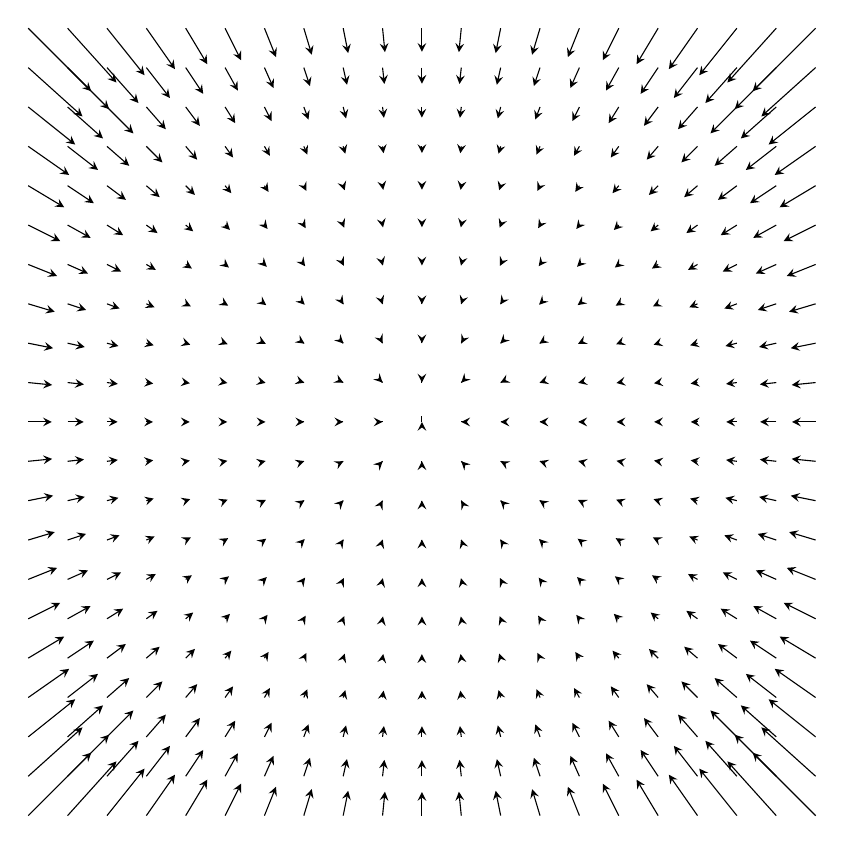
\begin{tikzpicture}[scale=5]

\def\ka{-0.04}
\def\kb{-0.02}
\def\kz{0.94} % 0.8

\foreach \y in {-10,...,10} {
	\foreach \x in {-10,...,10} {
	\def\xx{(\x/10)}
	\def\yy{(\y/10)}

	\def\rr{(\xx*\xx+\yy*\yy)}

	\def\corr{(1.0+\ka*\rr+\kb*\rr*\rr)}
	\def\xd{\xx*\corr}
	\def\yd{\yy*\corr}

	%\draw ({\xx},{\yy}) -- ({\xd},{\yd});
	\draw [-stealth] ({\xx},{\yy}) -- ({\xd},{\yd});
	}
}

\end{tikzpicture}
\end{document}
}{fig:raddist}
\simplegfx{h!}{0.6\textwidth}{raddist}
{Barrel-type radial distortion: lines point from destination image pixels to locations to sample from in original image.
The distortion is significantly larger near the borders.}

\simplefig{h}{%
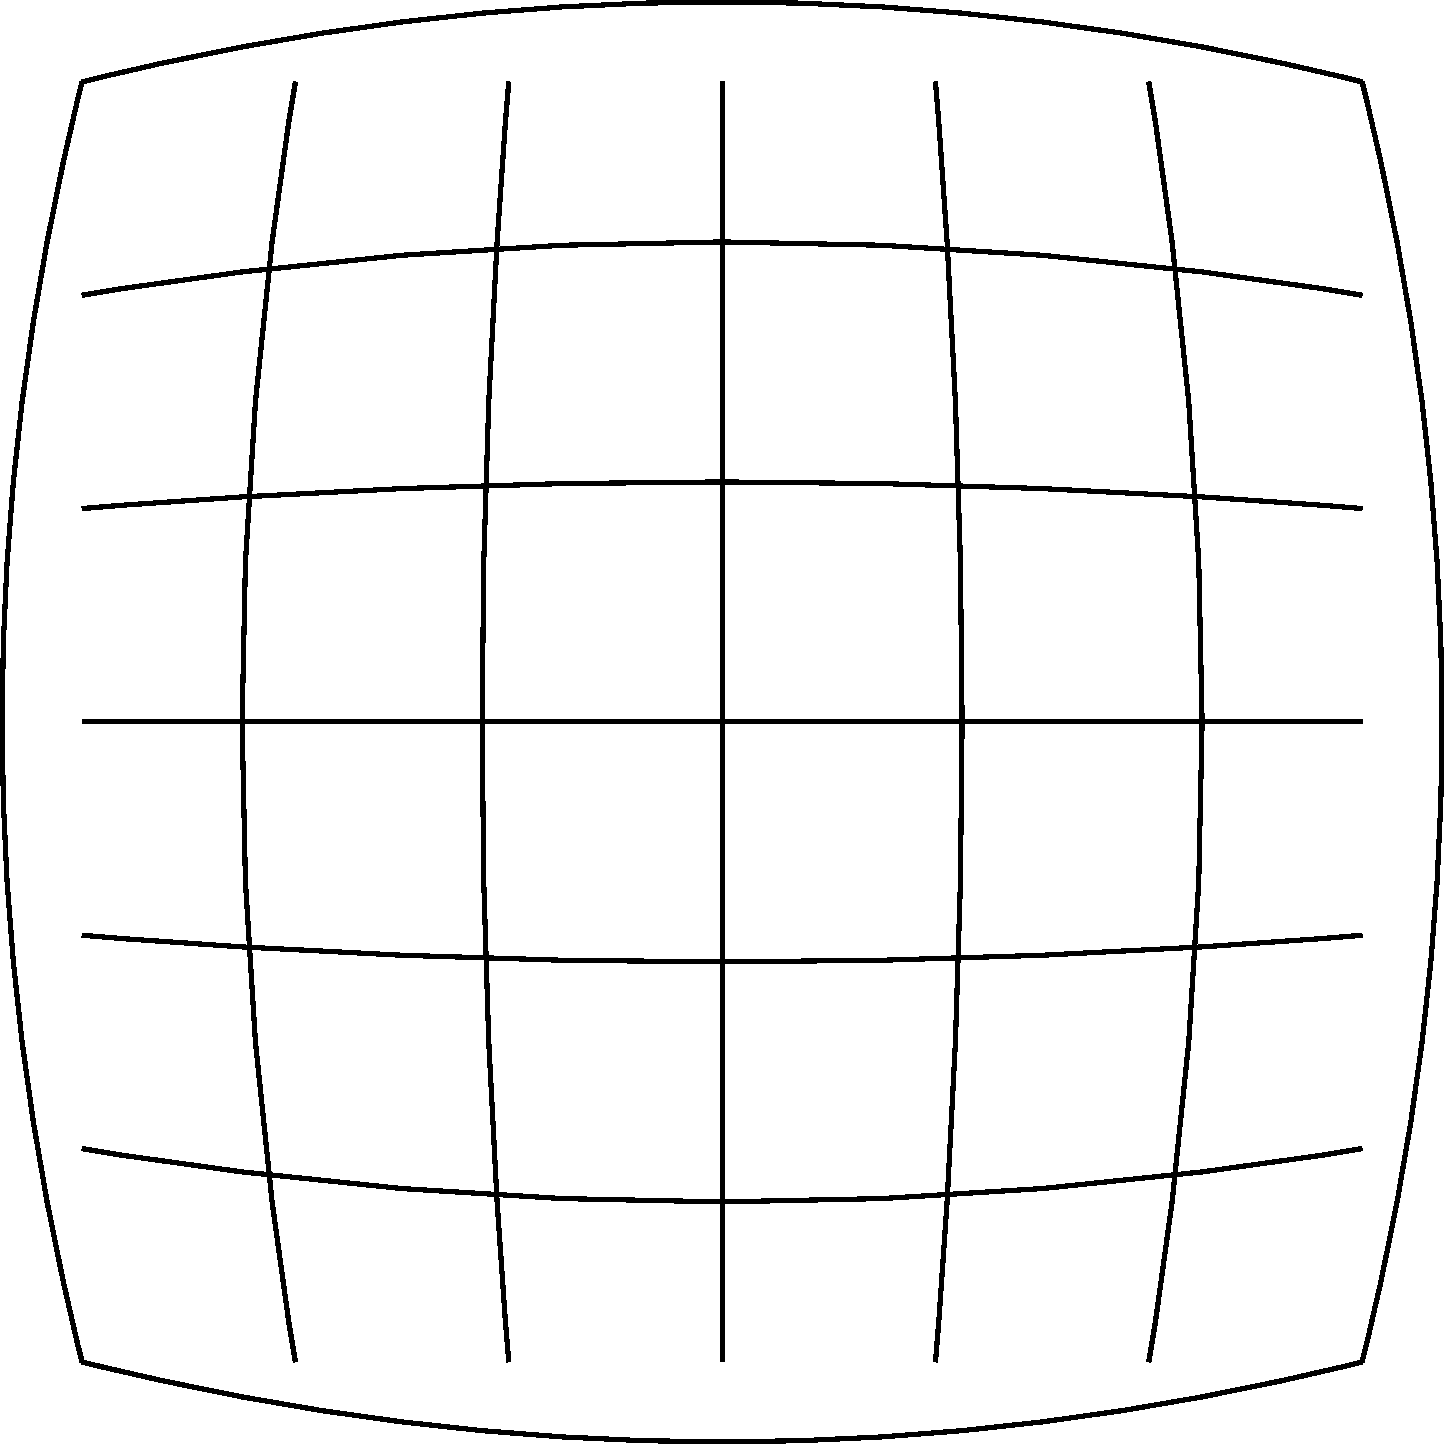
\includegraphics[width=0.2\textwidth]{gfx/barrel-distortion}
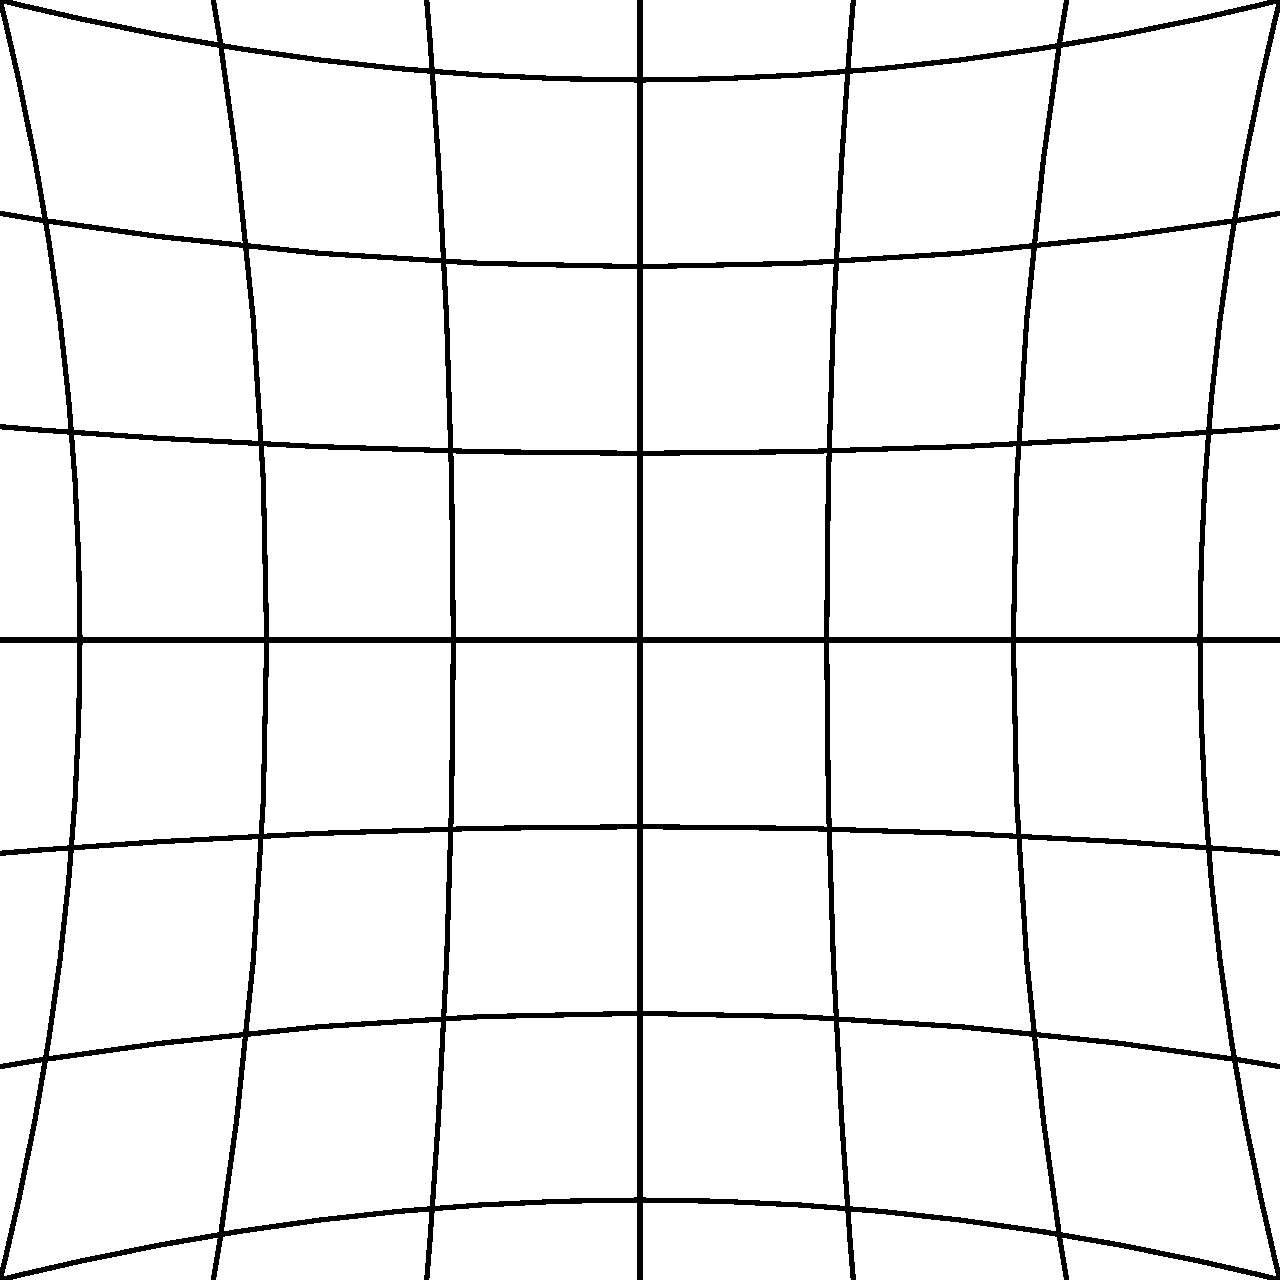
\includegraphics[width=0.2\textwidth]{gfx/pincushion-distortion}
}{fig:distortions}
{Barrel (left) and pincushion distortions that would show up in an image of a grid of straight lines. For a lens with no distortion, the lines would not be curved.}

Distortion should be corrected in software, as the following stereo algorithms assume that the images are free of nonlinear errors, i.e. straight lines in the world should remain straight in 2D images after the projective transformation.
%In particular, image rectification (discussed later in \ref{sec:rectification} won't work if this straightness does not remain; the assumption that similar features should be found on horizontal lines wouldn't hold on distorted images. \cite{hartley03multiview} 

The radial correction proposed by Brown \cite{brown1966decentering} and used by e.g. the OpenCV library \cite{opencv} to create a new image of the original pixel values at new positions is

\begin{align} \label{equ:radialdist} \begin{split}
	x_{corr} &= x(1 + k_1 r^2 + k_2 r^4 + k_3 r^6)\\
	y_{corr} &= y(1 + k_1 r^2 + k_2 r^4 + k_3 r^6)
\end{split} \end{align}

% (XXX some software does this in a different way (inverse of this, maybe?)

% TODO: illustrate pixel movements, such as in a vector field likein matlab toolbox

Trucco and Verri \cite{trucco1998introductory} use only the two first coefficients. For tangential distortion, the correction has the following form:

\begin{align} \label{equ:tangdist} \begin{split}
x_{corr} &= x + (2 p_1 x y + p_2 (r^2 + 2 x^2))\\
y_{corr} &= y + (2 p_2 x y + p_1 (r^2 + 2 y^2))
\end{split} \end{align}

In eq. \ref{equ:radialdist} and \ref{equ:tangdist}, $x$ and $y$ are the original coordinates in the distorted image, $x_{corr}$ and $y_{corr}$ are the corrected ones, $k_1$, $k_2$, $k_3$, $p_1$ and $p_2$ are coefficients specific to the distortion, and $r$ equals to the distance to image center where the optical axis hits, located at $(x_c,~y_c)$:

\begin{equation}
r = \sqrt{(x - x_c)^2 + (y - y_c)^2}
\end{equation}

The image size is often normalized such that the coordinates $x$ and $y$ range from $-1$ to $1$, making the distortion parameters universal for all image resolutions.

Because digital images consist of a discrete pixel array, the pixel coordinates given by the undistortion do not necessarily lie on exact pixel positions;
the sampling should then interpolate between neighboring pixels, instead of taking the nearest color.

%---

%Perspective distortion something something viewer location.
%Normal TV is usually watched at the distance of twice the screen diagonal.
%At this location, the scene looks normal when taken with a normal lens.
%A wide-angle scene then looks normal when viewed at a nearer distance. \cite{wilson2004anton}

% 14:01:55 <naavis> Kai sillä yritetään emuloida sitä, että katsojan paikalta se leffan kuvakenttä vastais sitä että valkokankaan tilalla on ikkuna.

% }}} optics

\subsubsection{Image sensors} % {{{

% intro: film vs sensor

Historically, photographs were saved on a photosensitive film.
With digital cameras, a rectangular electrical sensor replaces the film.
The sensor consists of a uniformly spaced grid of small pixel sensors built as an integrated circuit package.
A pixel, or picture element, represents a single dot on a film; when combined, the dots form a larger picture.

% digital pics

Digital pictures on a computer are commonly represented as rectangular arrays of numbers, or \emph{raster images}.
Each number describes the intensity of a single dot on a specific location.
For a single intensity value per pixel, a grayscale picture would be obtained.

Color pictures are described with more intensity channels than one, in e.g. RGB space, the way that most parts of a computer use for describing colors.
A single RGB color encodes the values of red, green and blue separately.

% sensors

The rectangular image sensor senses the amount of light hitting each pixel and encodes it to an electrical signal.
The signal is digitized to a brightness value and the camera saves all the pixel values to a file in mass storage.
There are two major sensor types: CMOS (Complementary Metal-Oxide Semiconductor) and CCD (Charge-coupled Device).
CMOS is the type used in most still cameras because of its lower price.

%It has some technical disadvantages, considering movie recording.
CCD captures a whole image frame at once (``global shutter''), while CMOS reads the sensor a single row at a time, resulting in an effect called ``rolling shutter'' \cite{todo:cmos}.
CCD has other issues, such as bleeding a strong light source to surrounding pixels and interlacing, i.e.~alternating in reading only odd and only even rows in consecutive frames.

% noise

As all electronic circuits, also image sensors are subject to signal noise.
Each pixel receives a more or less random level of signal that shows up as random additive brightness, noticed usually only in low light conditions as its power is much less than the actual brightness level of the light.
Black areas suffer from noise more than bright areas.
Noise increases also with sensor's signal gain, or ``exposure sensitivity'': also digital cameras use the ISO system designed for film speed.
More sensitive sensor needs less light to produce a bright-looking image by amplifying the signals more before digitization.
This amplification also amplifies the original signal noise, which is why the gain level should be kept as small as possible and the amount of light entering the sensor as large as possible.
This means using bright lights in the imaged scene or a longer exposure time.
Longer exposure time influences more motion blur, though.

% sensor movement

Some cameras use image stabilisation by moving the sensor around, as opposed to moving the optical elements inside the lens.
In any case, image stabilisation should be turned off for reconstruction because it affects the calibration: if any element in the image acquisition path moves, calibration parameters also change.

The sensor also moves when a camera uses a sensor cleaning mechanism with ultrasonic vibration motor on the sensor.

% colors

A single pixel sensor acquires all light hitting it, independent of the wavelength.
Two different methods to retrieve the red, green and blue color bands for each pixel are common in color cameras.
The most common method that most cameras use is to interleave red, green and blue in a single sensor by filtering the wavelength that can pass a pixel with a colored film over the sensor, with a special repeating pattern.
The missing values for other colors bands are interpolated from surrounding pixels.
The most popular interleaving pattern is the Bayer filter, illustrated in figure \ref{fig:bayerpattern}.
Other arrangements of red, green and blue are also common, and it is not mandatory to use these three colors; there exist filters for e.g. cyan, yellow and magenta too.

Another way is to retrieve the three channels with three different sensors, one for each wavelength band, and to guide the light to them with prisms and filters; this is obviously more expensive than a single sensor but results in a more accurate picture as there are all colors available for each pixels.

\simplefig{h}{\bayer{0.6}}{fig:bayerpattern}
{A small subsection of the repeating Bayer pattern, not drawn fully for better visualization. Each square is a single pixel; the grey area represents the image sensor. The gap between pixels is nonzero.}

% ???

Physical pixels cover less than the full area of a sensor, as there are gaps between them;
microlenses between the pixel sites direct the light hitting the gaps to the neighboring pixels.

% support electronics

Next to the pixel sensors and their amplifiers is digital logic for reading out the data and passing it through to an image processor.
Quality of this support electronics affects some properties, most important of which are analog-digital converter noise and dynamic range, and speed that the image is read out from the sensor.
A so-called raw image file can be saved with more expensive cameras contains the raw sensor data with very little processing done;
when a raw file is not used, the camera processes the image with device-specific correction filters and applies e.g.~white balance correction, and finally saves the image as a standard image file such as JPEG.

% }}} image sensors

\subsubsection{Shutter} % {{{

% shutter, why needed

An image sensor accumulates the received light and converts its intensity to electrical signals.
A static scene is imaged so that the sensor is exposed to the light passing the optics for a short time, keeping the camera and subject steady.
Electrical sensors can be ``cleared'' to black rather quickly (unlike an analog film that starts exposing immediately and the effect cannot be undone). Still, good quality cameras use mechanical shutters for photographs.
Because of the rolling shutter effect of a CMOS sensor, it is better to do the reset and readout phases when the sensor is not exposed to light.

% mechanical stuff

\simplegfx{h!}{0.5\textwidth}{focalplaneshutter}
{Focal plane shutter has two moving curtains to cover the sensor, opening it momentarily so that each pixel receives light for the same amount of time.
Top: initial position, sensor blocked.
Middle: first curtain moved away, sensor exposed to light.
Bottom: second curtain has moved to cover the sensor.
The shutter resets by moving back to the position in the top.
Modern curtains do not actually have whole planes but folding metal pieces to save space.}


A shutter is a mechanical device that blocks light to the sensor and can be moved quickly out of the way and back.
There are several types of mechanical constructions for shutters, depending on the application.
A focal plane shutter, used in most system cameras, is installed in front of the sensor.
It consists of two curtains that move to the same direction; one moves out of the way of the sensor to let light pass to it, and another moves to cover it back again when the exposure time has elapsed.
Figure \ref{fig:focalplaneshutter}.
A \emph{rolling shutter} effect is produced with very high shutter speeds, where the limit of curtain movement speed prohibits fully opened shutter and the closing curtain starts to move before the first has stopped, exposing only a narrow band of the sensor at a time.

A digital CMOS exposure and ``electrical shutter'' works like this too; the sensor is reset and read row by row sequentially; this produces a strong rolling shutter effect especially in short exposures and in video.

A CCD camera would not need a mechanical shutter, because the full image is read out at once.
Most still cameras have also a movie mode that holds the mechanical shutter open all the time, using the electrical shutter.

The mechanical shutter can last only a finite amount of actuations (50-200 thousand for a common system camera) as it wears out gradually.

%varying ccd charge time, ???
%

% vs frame rate

% other

When the camera or the imaged subject moves while exposing the picture, an object gets smeared along the movement on the image, an effect known as ``motion blur'': the image gets blurred where motion happens.

Video film cameras that capture each frame to a separate part of film used a spinning wheel with a window in it, called rotary disc shutter. \cite{wilson2004anton}
This rotates at a precise speed synchronized to the frame rate, displaying a for a consistent duration for each frame.
The size of the window constitutes to the amount of light and motion blur. Video is more discussed in the section \ref{sec:video}.

When taking a picture, the camera does not instantly start to expose the image.
Each camera has a specific \emph{shutter lag} that is the time that elapses between when the shutter button is pressed and when the shutter moves out of the way.
Some sources include in this term also the time for the camera to focus the lens and measure sensitivity settings which can be a significantly longer time.

Shutter speed has small variations over time when the camera ages and some parts wear out.
Some difference also exists among same camera model from factory variations.
Even a single camera cannot be exactly consistent in e.g. unpredictable firmware causes if it has not been taken into account in the design.
The variations among several cameras must be taken into account when using a flash unit instead of continuous light: the short duration of the bright flash of light should happen when all the cameras imaging the same scene have opened, but not yet closed, their shutters.

%Shutter lag (auto exposure/focus even in manual mode maybe?)

% }}} shutter

\subsubsection{Lighting} % {{{

In addition to multiple cameras at different locations and poses to encode a subject's geometry, a uniform and soft lighting is also required to minimize bright reflection difficulties in the texture.
A large variety of different studio lights are available in the market for different lighting situations, emitting either continuous light or short bright flashes.

% XXX pic of brightness constancy: same object from two views, patch windows
Because most reconstruction methods fundamentally assume a relatively diffuse lighting, a property called \emph{brightness constancy} (i.e. the brightness and color of a surface looks the same from all viewing directions), they perform poorly when a light shines off a surface so that its specular highlight is at a different geometric location in different images.

\simplegfx{h!}{0.7\textwidth}{brdfdiagram}
{BRDF of a surface is a function of surface normal $n$, light direction $\omega_i$ and viewing direction $\omega_o$.}

Some surfaces are more \emph{diffuse} than others.
Surfaces can be modeled as diffuse and specular components that are functions of light direction, viewing direction and sometimes spatial location on the surface.
Surface reflection models are described with a bidirectional reflectance distribution function, or BRDF. \cite{nicodemus1965dirreflectanceetc}

A distribution model of the surface's global or local microgeometry specifies how much light reflects in different surfaces. \cite{nayar1991surface} % XXX 1991 or -89?
Diffuse means a material that reflects light uniformly to all directions, depending only on the angle between the surface normal and light location, whereas more \emph{specular} surfaces are composed of a different microstructure that reflects light in a more mirror-like way and the surface brightness depends on where it is looked from.
Diffuse surfaces are called matte or Lambertian; they follow Lambert's cosine law (equation \ref{eq:lambertcosine} often used in computer graphics), a lighting model, shown in figure \ref{fig:lambertcosine}. \cite{lamberttodo}
A Lambertian surface's BRDF is constant among the viewing direction.
Specular highlight or specular reflections refer to a mirror reflection of the lamp on the imaged surface.
Surfaces modeled in computer graphics are often relighted with functions of surface normal and light and view directions, given as unit vectors, as in figure \ref{fig:brdfdiagram}.


\begin{equation} \label{eq:lambertcosine}
	I_D = L \dot N I_L = |N| |L| \cos \alpha = \alpha
\end{equation}

[Some specular lobe picture here and definitions of the rendering equation, probably.]

Commonly used but vague terms such as ``soft'' and ``hard'' lighting refer to the size and power of light sources: bright spotlights are hard, and larger and relatively less bright lamps are soft.
Softness can be added by increasing the light's area while holding its power constant, such as reflecting a light off a large surface or adding a white cloth between it and the imaged subject.
Effects of a soft versus hard light are illustrated in figure \ref{fig:lighthardness}.

Powerful flash light sources use usually a gas-filled tube (Xenon) that is excited with high voltage to produce a short, bright burst of light.
Flashes are good for portrait photographers because the subject sees the bright light only for a short moent; thus, the light does not annoy the subject.
Short bursts of light are also good for stopping motion: motion blur happens when the camera sees movement over time, but it only sees the light that enters the scene and reflects to the lens.
If light enters the scene only for a short while, no motion blur is possible.

Consumer flashes output a short spike of light, with a duration of a few milliseconds.
When attached to a flash, many DSLR cameras refuse to use a shorter exposure time than around 1/200 s.
There is a limit on the movement speed of the shutter mechanics.
A short exposure is taken so that the opening and closing curtains move at the same time, exposing only a short band of the sensor to light at a time.
The flash does not usually last long enough for the whole sensor to expose, resulting in a partly bright and partly dark image.
Some more expensive models support ``X-sync'', where several shorter flash bursts are fired in sequence, resulting in a longer overall light pulse.

%dark contact lenses if available (remedy)

%bodies' own flashes maybe not uniform enough; too many flashes i guess

%softbox or umbrella

%Polarization filter

% }}} light sources

\subsubsection{Image download} % {{{

% data path intro

The image information travels from the subject through the optics to the image sensor's surface, via an analog/digital converter, the camera's processor(s) and finally to a memory card or straight to a computer's storage via a wired or wireless connection.
Many parts in this equation contribute to the rate of which the images can be taken, usually measured in frames per second (FPS).

% fps

An average DSLR can achieve around five frames per second of full resolution footage, while more expensive models can reach over 10 FPS.
A digital still camera can often record video too, at a lower resolution and a higher FPS.

% sample speed calculations

For example, recent Canon consumer DSLRs such as 650D and 700D feature an 18 megapixel CMOS sensor having a resolution of 5184 by 3456 pixels and a 14-bit analog/digital converter, resulting in approximately 31 megabytes of raw data per frame.
For a moderate 5 FPS, the sensor generates thus about 155 MB of data per second, as shown in equation \ref{equ:canonmbfps}.

\begin{equation}
	5\frac{1}{s} * 5128 * 3456 \text{px} * 14 \frac{\text{bit}}{\text{px}} \approx 1240 \frac{\text{Mbit}}{s} \approx 155 \frac{\text{MB}}{s}
\end{equation}

% files

The raw files saved by DSLR cameras are compressed in a proprietary lossless format and contain also metadata about certain camera settings.
Lossless compression maintains image quality and reduces file size depending on the complexity of the frame.
Some manufacturers encode the brightness values through a lookup table, and it's common to use a compression scheme known from standard file compressions, or a specific lossless image compression.

Video files are almost always saved in a lossy video format, the H.264 format being common for recent cameras.
Common bitrate for a full-hd (1920 by 1080 pixels) 24 FPS video is about 5-6 MB/s maximum.

% storage

Files are commonly stored to an internal memory memory of the camera, to a removable memory card, or directly to a PC via a cable.
Files not directly transferred to a PC can be moved later by removing the memory card, or via USB connection that most consumer cameras support.

Memory cards used by consumer grade cameras (CF, SD) can support speeds up to 125 MB/s and capacities in tens of gigabytes.
The speed of USB 2.0 high-speed specification is 480 Mbit/s; bus protocol's overhead limits effective data throughput to around 80 \%.
Computers typically have several USB hosts each capable to the maximum transfer rate.
To speed up download from multiple devices, the devices should be connected evenly to all hosts to fully divide the workload.

Machine vision cameras use a higher speed connection, such as the newer USB 3.0, IEEE 1394 (FireWire), gigabit Ethernet or Camera Link to achieve realtime lossless transfer of high-resolution images.
For example, the 1 Gbit/s Ethernet connection can transfer a raw 12-bit full-hd stream at

\[
	\frac{1 \text{Gbit}/s}{1920 * 1080 \text{ px} * 12 \text{bit}/\text{px}} \approx 43 \frac{1}{s}
\]

where Gbit is $1024^3$ bits.
Manufacturers can use some kind of compression to achieve higher rates.

%http://majid.info/blog/is-the-nikon-d70-nef-raw-format-truly-lossless/

% }}} image download

\subsection{Video} % {{{

Video is ordered electronic pictures displayed one after another.


%Hox ALL-I (intra) vs. IPB (intra-predict-bidirpredict)

Humans perceive motion when a previously seen object is seen again in a nearby location.
Current digital video technology encodes motion in a sequence of still images, usually displayed in constant rate.
Three dimensional motion is generally no different: it is encoded as discrete poses in sequence.
In order to do motion capture in stereo vision, video material from two or more of cameras is used to initially capture a sequence of still photos.

% }}}

\subsubsection{Sequence of frames} % {{{ or: video is frames

When scanning a scene continuously, a camera grabs frames using the same principles as in photos, but does it in sequence, at a speed that is called frame rate.
Each picture of a video stream is called a frame.
In interlaced video, two frames make up a whole picture that covers all pixels.
Interlacing alternates between odd and even lines to increase update rate, and was invented for cathode ray tube (CRT) displays.
Many CCD video cameras still produce interlaced stream, because it is cheaper to manufacture.
Video that contains full frames only is called progressive.

In movies, the shutter is often open deliberately so long that fast motion is blurred, because it is considered aesthetically pleasing to human eye; even though the motion is blurred, more temporal information about the scene movement is encoded per frame than when exposing infinitesimally short frames, at the expense of spatial resolution.
A common shutter speed relates to frame rate such that a frame is exposed half the time between frames.
\cite{wilson2004anton}
For sharp images that are preferred in 3D reconstruction, motion blur should be avoided.
Ideal exposure time would be infinitesimally short, but practically the shortest possible cannot be used becauses of the amount of light available.

Film cameras and some professional video cameras use a rotary disc shutter that has an opaque 180 degree sector.
This is why having half the exposure time of frame rate is sometimes called ``180 degree shutter''.
While the light is blocked, film is mechanically advanced to the next frame.
Digital video analogously downloads data from the image sensor and clears it during this time.

% }}}

\subsubsection{Frame rate effects} % {{{

For a same subject, a higher FPS usually means better stopping of motion because of shorter shutter speed and less movement between frames.
For optical flow computation, a long enough time should be passed for reliable motion vectors, though.

Interlaced video was invented to increase the update speed of cathode ray tube (CRT) displays, reducing apparent flicker.
Progressive video means a format where each picture is a full frame.
Interlacing has twice as high update speed as progressive, because each picture encodes only half of the images.
The pictures alternate between odd and even lines only, resulting in tearing artifacts when imaging moving subjects (shown in figure \ref{fig:interlacetearing})
Some CCD sensors employ a technology that scans the image in interlaced frames.

\simplegfx{h!}{0.9\textwidth}{interlace}
{Interlaced scanning. From left to right: even lines only, odd lines only and full picture combined. Picture not in scale, only 20 lines used.}

Consumer video cameras and video-capable pocket cameras and DSLRs typically offer several choices of frame rate. Traditionally, the movie industry has used 24 FPS; 25 (PAL) and 30 (NTSC) are common alternatives used in TV broadcast, some cameras being capable to twice the speed on a lower resolution.

Actual FPS in camcorders is slowed down by a factor of 1.001 because of historical reasons relating to black and white / color TV backwards compatibilities.
30 and 24 FPS refer often actually to approximately 29.970 and 23.976 FPS, respectively.

Externally triggered cameras can be configured to record at any arbitrary speed, as long as it's in the limits of the camera speed capabilities.
Synchronized machine vision cameras do not record video on their own, but instead just listen to a synchronization signal and output frames on its rate, that frame grabbers on a computer read and store.

% }}}

\subsubsection{Frame rate vs. shutter speed} % {{{

\simplefig{h!}{
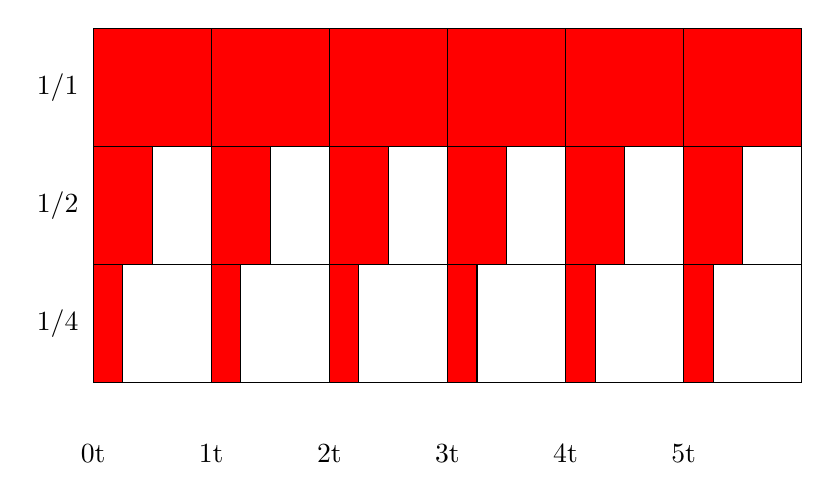
\begin{tikzpicture}[scale=1.5]
	\def\nframes{5}
	\draw (0,0) rectangle (6,-3);
	\draw (0,-1) -- (6,-1);
	\draw (0,-2) -- (6,-2);
	\foreach \x in {0,...,\nframes} {
		% time ticks
		%\draw (\x*1, 0) -- (\x*1, -2.5);
		\node at (\x*1, -3.6) {{\x}t};

		% exposure blocks
		\draw [fill=red] (\x*1, 0) rectangle (\x*1+1.0, -1);
		\draw [fill=red] (\x*1, -1) rectangle (\x*1+0.5, -2);
		\draw [fill=red] (\x*1, -2) rectangle (\x*1+0.25, -3);
	}
	\node at (-0.3, -0.5) {1/1};
	\node at (-0.3, -1.5) {1/2};
	\node at (-0.3, -2.5) {1/4};
\end{tikzpicture}
}{fig:shutterspeed}
{Shutter speed compared to frame rate. For an always open shutter, the camera records everything. 1/2 is a ``normal'' rate, 1/4 resulting in slightly less motion blur.}

What happens when the shutter is closed cannot be recorded.
The Nyquist-Shannon sampling theorem states that events higher than half the sampling rate cannot be distinguished from the signal.
In reality, repetitive motions rarely happen in reconstruction videos, but the fact that information about the subject between frames is lost cannot be circumvented.
Normally, motion is simply interpolated between views in different frames or simply the last frame is used, if playback happens at a different rate from the recording.
For a large displacement, this interpolation can be inaccurate enough to need manual fixing.

Motion blur encodes more information about object travel but gets less precise by time.

slowmovideo 
\cite{eugster2011slowmovideo}

DSLR video modes use almost the sensor's full size but skip some of its lines when recording video, getting the same field of view as still images but sometimes resulting in significant aliasing patterns with certain subjects with high frequency information.
Line skipping is depicted in figure \ref{fig:lineskipping}.
The color filter array makes the problem even worse.

\simplegfx{h!}{0.9\textwidth}{lineskipping}
{Line skipping in a video camera. Left shows a part of the full sensor and its bayer pattern; on the right, only every third line is captured. (TODO: draw a cleaner and not stolen pic)}


% }}}

\subsubsection{Multi-camera synchronization} % {{{

%Time offset / drift / jitter / lockstep

Synchronized recording of multiple view video is more complicated than shooting still photos simultaneously.
Cameras should be synchronized, i.e. locked to hold their shutters open at the same time during each frame.
When cameras open their shutter in a different time, they effectively shoot a different scene (assuming moving subjects in the scene), breaking one of the most fundamental assumptions of stereo vision: that the images encode geometrically same objects.
This can be compensated to some degree with optical flow if hard syncing is not possible. \cite{bradley2009synchronization}

Synchronization issues can be divided in three major errors, assuming N cameras each having its own video file: offset, drift and jitter.
Offset is the time difference relating start time of two streams: for camera $A$ at each frame index $t_{Ai}$ for an increasing $i$, and camera $B$ at $t_{Bi}$, a constant $e$ is added, as in eq. \ref{eq:timeoffset}:

\begin{equation} \label{eq:timeoffset}
	t_{Bi} = t_{Ai} + e
\end{equation}

Drift is a property of one single camera that advertises to record at some speed and actually works at some other speed, similarly, shown in eq. \ref{eq:timedrift} for cameras $A$ and $B$, constant $e$:

\begin{equation} \label{eq:timedrift}
	t_{Bi} = t_{Ai} + e * i
\end{equation}

Jitter is the random difference between frames for a same camera, in equation \ref{eq:timejitter}, when $e$ changes:

\begin{equation} \label{eq:timejitter}
	t_{Bi} = t_{Ai} + e(i)
\end{equation}

For an actual video camera, drift and jitter are negligible; offset originates from pressing record buttons at a different time and from the camera's internal processing before the recording actually starts.
If the cameras take pictures only when instructed, such as machine vision cameras, a clock generator becomes another source of jitter.
Many consumer compact cameras support a preview feed for individual frames when connected to a computer; the feeds can be useful for previewing but jitter becomes too significant because cameras are not designed with this in mind.
If the offset between two cameras is not an exact multiple of the frame speed, they effectively cannot have any frames that would display exactly the same scene.

Frame accurate offset sync with clapperboards works by matching the clap sound to visual cues in the video.
Cameras that record audio to the same video file do not need visual cues and can be synced together by matching the sound stream only.
This is the method used in making movies when editing a final version with multiple cameras used.
It still leaves at most half a frame lag between the camera sequences; this is illustrated in figure \ref{fig:syncproblems}.

Synchronizing all the cameras that shoot the same scene might be a big issue in practice, depending on the gear used.
Professional grade cameras can be synced to a single clock generator, so that they all operate on the same frequency (i.e. no drift) and phase (i.e. no offset).
The same method is used when shooting with machine vision cameras that have external trigger input.
This still leaves a small phase difference (offset) caused by unequal transmission paths from the clock generator.
Synchronizable camcorders are very expensive, and consumer-grade hardware usually lacks all possibilities for proper sync.

\begin{verbatim}
Drift

normal   |   |   |   |   |   |   |
drifting |    |    |    |    |    |
         0t  1t  2t  3t  4t  5t  6t time -->


Jitter

normal   |   |   |   |   |   |   |
jitterin |    |  |   | |      |    |
         0t  1t  2t  3t  4t  5t  6t time -->
\end{verbatim}

%Often used techniques are starting flash (does not need an audio track) [REF], clapperboard [REF], strobe sync'd to fps, genlock.

\simplefig{h!}{
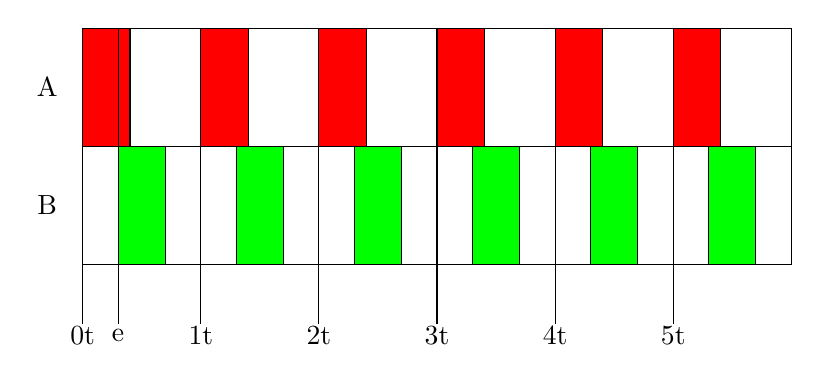
\begin{tikzpicture}[scale=1.5]
	\draw (0,0) rectangle (6,-1);
	\draw (0,-1) rectangle (6,-2);
	\foreach \x in {0,...,5} {
		\draw (\x*1, 0) -- (\x*1, -2.5);
		\node at (\x*1, -2.6) {{\x}t};

		\draw [fill=red] (\x*1, 0) rectangle (\x*1+0.4, -1);
		\draw [fill=green] (\x*1+0.3, -1) rectangle (\x*1+0.3+0.4, -2);
	}
	\draw (0.3, 0) -- (0.3, -2.5);
	\node at (0.3, -2.6) {e};
	\node at (-0.3, -0.5) {A};
	\node at (-0.3, -1.5) {B};
	% P, Z
\end{tikzpicture}
}{fig:syncproblems}
{Video phase difference, i.e.~offset.
Red rectangles illustrate exposure times of camera A, green rectangles the same for camera B.
Frame period is t, and the cameras have a constant exposure time offset of an arbitrary e.}

Faster frame rate encodes information more often, which is preferable as longer distances of pixels of same objects are more difficult to match when tracking objects; faster shutter speeds help to reduce motion blur.
Fast shutter (i.e.~short exposure) obviously needs to be compensated by using more sensitive sensors or more light to get equivalently bright images.
Short exposure becomes problematic if the light source is a flash instead of continuous, if camera offset can be more than the exposure; the flash might illuminate only some cameras while others expose when the flash is not lit.

Video recording and motion tracking are best considered orthogonal issues; while a single static case can be scanned in three dimensions, so can be also each frame of a sequence, separately.
It might not be computationally feasible in all use cases, though, because the reconstruction must be started all over again for each frame and the topology is uncorrelated between the frames.
% Assumptions that the scene is locally almost the same can help and speed up computations. [?]

%Section \ref{sec:tracking} will 

% }}}

\subsubsection{Encoding quality} % {{{

Raw video consumes too much data to be feasible to use normally.
Thus, a range of compression algorithms have been invented, most of them lossy.
Reconstruction from frames extracted from a compressed video can not be as good as from separately saved stills.

Compression introduces loss of detail and artifacts typical to each algorithm, often visible as blocks or blurring.

Some expensive cameras can record raw video, and others can be tricked to that.
Canon DSLRs can be ``hacked'' to dump the raw stream to a memory card, but only some models support the faster CF memory cards that can keep up with the amount of data.

% }}}

\subsection{Digital camera types} \label{seq:cameratypes} % {{{

% intro on camera types and wanted options

This section lists the most common types of cameras available for the typical consumer and their properties that have most effect on reconstruction quality.
Good properties are image quality, configurability, ease of use and low price.
Technical qualities usually get better with price.
For a multi-camera setup with a restricted budget, low price is one of the largest advantages.
On the other hand, large amounts of manual work should be avoided if possible; cheaper devices are usually more clumsy to use.

% comparison on some properties

Consumer cameras have good availability, but they are targeted for artistic photographs instead of science.
They are divided roughly in two categories: DSLRs and compact (pocket, or point-and-shoot) cameras.
Industrial cameras for machine vision are more controllable and contain no unnecessary bulky parts, but are more expensive, difficult to acquire and need proprietary control tools.

In general, good technical properties are deep depth of field, light sensitivity, high resolution, and short distance to the subject.
Practical features also count, such as availability of external power supply instead of batteries.
Some technical properties of cameras that affect quality the most are listed below.

\begin{itemize}
	\item Sensor size: For an equivalent resolution, smaller sensor leads to deeper depth of field. Larger sensor requires a closer target or longer focal length for filling the frame, which leads to shallow DOF.
	\item Pixel size: larger pixels gather more light; they increase the sensor size, though.
	\item Pixel count: resolution gives more texture accuracy.
	\item Focal length: smaller focal length results to less distance needed between camera and the subject, leading to smaller rig footprint.
	\item Aperture size: Smaller aperture leads to deeper depth of field, but requires longer exposure times for equivalent amount of light.
	\item Fixed focal length lens (prime lens): less moving parts means better calibration.
	\item Remote control: changing parameters such as exposure time for all cameras must be automatic.
\end{itemize}

All the properties should be looked as a whole; especially large pixel count does not necessarily imply better pictures if the optics is not good enough.

Resolution, or pixel count, is declared in million pixels, or megapixels (Mpix).
Resolution and image size are related via pixel size that declares the physical size of one photosite on the sensor.
Pixel size is described as the length of one side, and the pixels are almost always square.
Newest consumer DSLRs can have a resolution of up to 20 megapixels.

%camera position disparity

% XXX pocket/compact camera naming

% sensors

Typical sensor sizes for different camera types are:

\begin{itemize}
	\item System cameras use ``full-frame'' (36x24 mm) or APS-C (1.5-1.6x crop of full frame, i.e.~about 22x15 mm), resolution usually over 15 Mpix with pixel size at about 5 micrometers
	\item Compact cameras use a small sensor; sizes vary a lot but are approximately 1/2.3" (6.2x4.6 mm), resolution about 10 Mpix
	\item Smartphones use sizes between 1/3"-1/4" (less than 4.8x3.6 mm), resolution between 3 to 8 Mpix
	\item Sizes used by industrial machine vision cameras vary by application, in 5 to 10 mm range having resolutions from 0.5 to over 10 Mpix.
\end{itemize}

DSLRs usually benefit from bigger pixel size to get better light sensitivity, and the shallow DOF is commonly appreciated because of its artistic value.

%sensor vibration to remove dust -> sensor position not very fixed \cite{rieke2009}. % TODO MEASURE!
%no image stabilizer in sensor or lens \cite{photogrammetry.doc}
%ring flash bending the lens assembly if attached to it \cite{rieke2009}.

% http://www.agisoft.ru/forum/index.php?topic=1411.60

% lenses
% MILC/CSC?
System cameras (DSLRs, MILCs) have by definition interchangeable lenses, while cheaper compact cameras, phones and webcams are designed for a single lens that cannot be removed.
Compacts accompany a zoom lens; zooms are more complex systems and therefore more expensive to reach a good image quality.
Calibration is also a problem with moving elements that rarely align to precisely same setting.
With a DSLR lens that has a moving mirror and shutter, the mechanical vibration could move the zoom lens each time a little, changing the lens parameters.

System cameras have a large selection of fixed focal length (``prime'') lenses.
The lack of zoom of a prime lens is acceptable in a lab environment, where the distance to the subject can be adjusted as necessary.

Lens sharpness is defined via their performance to high contrast, measured with modulation transfer function (MTF).
Perceptual pixel count relates to lens contrast; a high pixel count sensor for a poor quality lens is only useful for observing the lens defects.

Rieke-Zapp et al \cite{rieke2009evaluation} address several problems in camera calibration and imaging quality.

% shutters

System cameras usually use a mechanical focal plane shutter, and SLRs have an additional mirror to direct the image to a viewfinder.
The mirror moves away when exposing the image.
Some compact cameras have a leaf shutter in the lens, but many use digital shutters, resulting in rolling shutter artifacts for moving subjects.

% storage speed
Storage size and speed and camera processing power in general follows camera price.
High-quality capture of short motions is aided by continuous burst mode that can achieve anything between 2 and over 10 frames per second, depending on camera model and price.
Professional-level DSLRs can handle over 10 continuous raw full frames per second, while entry-level DSLRs handle around five;
compact cameras are generally slower.
Overall storage speed is determined by several factors.
Immediate readout speed from the sensor is affected by sensor, A/D converter and processor speed.
Writeout to the mass storage medium is done from the camera's RAM, which can usually hold several pictures.
Top storage medium speed varies by price.
Best CF cards (used only in professional DSLRs) can write at about 150 MB/s, while SD cards reach 90 MB/s, but camera bus drivers usually only achieve 20-40 MB/s. % TODO canon, magic lantern, uhs-i

Reading the pictures to a computer can be done via USB or a memory card reader; the latter method is inconvenient as the card must be removed from the camera and placed to a reader manually.
A card reader is usually faster than a camera directly though.

Industrial cameras usually have temporary memory for only one frame that is read out immediately.
For high speed video, this needs relatively large amounts of auxiliary hardware to save the raw frames, roughly a gigabit connection per camera, plus hard drives that can save the data fast enough.

% software support
Major consumer manufacturers provide software development kits (SDK) for controlling their cameras remotely at some degree, and industrial devices always have an accompanying SDK.

Consumer SDKs by the largest manufacturers such as Canon, Nikon and Sony are relatively capable and can change any property of the camera that can be changed manually, e.g. aperture, shutter speed and ISO rating.
They can also take pictures remotely and download them, and display a live view preview for some models.

Gphoto2 is a free software alternative that aims to control camera's file system and properties, independently of camera maker and model.
It has mature support for over a thousand cameras and camera-equipped mobile phones.
It consists of two parts: a software library that can be embedded into other programs, and a command-line tool for using the library directly.

For Canon DSLRs, there is also a third-party open source firmware add-on that aims to enhance the user interface, and to hack additional experimental features such as RAW video recording.
Another third-party add-on is the Canon Hacker's Development Kit (CHDK), a firmware for Canon's compact cameras.

For machine vision cameras, manufacturers provide their own software packages, in addition to sometimes specifying that the camera complies to a standard.
The standards specify data formats, image streaming and control methods.
Key standards for industrial cameras are:

\begin{itemize}
	\item Camera Link, partly proprietary (but significantly reverse-engineered) serial transfer protocol with special cable and connector types
	\item GigE vision, standard interface for video data over gigabit Ethernet connection; licensed so that writing open source software based on the standard is not officially possible
	\item IIDC/DCAM, Instrumentation \& Industrial Digital Camera or 1394-based Digital Camera Specification, data format standard used in IEEE 1394 (FireWire) cameras; an open specification
	\item USB3 Vision, a standard for the USB 3 bus
\end{itemize}

A standard-compliant industrial camera enables to use readily available software, reducing the need for in-house software and protecting from vendor lock-in.
Some of the largest manufacturers that offer standards-compliant cameras are Point Grey, Basler, Allied Vision, Imaging Source.
Coriander \cite{coriander} is a free user interface for controlling IIDC cameras.

% triggering
For a multi-camera setup, reliable remote trigger is important.
It must be possible to ``press'' the shutter release remotely to take a picture (or to start video recording).
Industrial cameras are designed to be remotely controllable, and system cameras have input sockets for remote trigger buttons.
Others have limited offer, mainly supporting infrared remote if anything.
As a special case, CHDK supports a hacked remote release via USB port.

% camera comparison

Summarizing for the most popular camera types in the market:

\begin{itemize}
	\item System cameras with bigger sensors are good for artistic still photos, have excellent configurability with lots of hardware available, and decent software support. Designed for single pictures, these often lack in video features.
	\item Industrial machine vision cameras have both small and large sensors, support interchangeable lenses and need a lot of additional hardware, and custom or expensive software to control
	\item Camcorders are only good for video recording, have properties for film editing but have poor resolution for still pictures. Electrical shutter, some interlaced. Deeper DOF. Only pro devices have external sync.
	\item Compact cameras, designed for the general public for all-purpose point-and-shooting are cheap, have non-changeable zoom lenses and are in general slower. Some do shoot RAW images. Most lack external AC supplies. Resolution is less than in system cameras, and high-resolution cameras perform worse in low light because of smaller pixel size.
	\item Others (smartphones, webcams) have poorly documented features and bad lenses that are hidden by overly compressing jpeg images.
\end{itemize}

In addition to multiview stereo, there are cameras that can capture depth directly.
Laser range finders are common in automation industry, and have great precision and high price.
Active infrared cameras such as the Kinect (sensor manufactured by PrimeSense) project an infrared pattern of dots to the camera's view and estimate depth in coarse blobs, resulting in an easy-to-use depth camera but poor accuracy.
Light field cameras such as the newer Kinect 2 have a better spatial accuracy but not yet an established reliable software state.

% }}} camera selection

\clearpage
\section{Static 3D reconstruction}

%[1] Shape and motion from image streams under orthography: A factorization approach

% kruppa eqs
% active vs. passive http://en.wikipedia.org/wiki/3D_reconstruction

%algebraic vs geometric error

% previous work! implemented algorithms

Close range photogrammetry, stereopsis, isolated object, camera resectioning

Pairs vs overlap? bradley: pairs

% TODO: intro paragraph(s)

\subsection{Imaging methods} % {{{

% separate part or part of 3d reconst intro? or combine to intro?

some basic stuff about how 3d structure can be recovered with many different means (i.e. different camera types): light field, structured light, laser scanner, multiview stereo

- every Nth frame free of patterns for texture extraction (zhang snavely curless 2004)
- maybe not fast enough with common cameras

% }}} imaging methods

\subsection{Coordinate systems and transforms} % {{{

% (XXX rename?)

%Homogenous point description here, [dubrofsky] homography estimation is nice, also refer hartley/zisserman

%Homography definition (mapping of points and lines in $P^2$) / panorama homography

The previous imaging section described how to record a view of a scene with a camera. From now on, the term camera refers to a particular camera configuration, which can be a single physical camera moved to different locations.
No optical system is assumed; at this point, the camera is reduced to the pinhole model \ref{sec:pinhole}.

% FIXME: describe more of these in pinhole and less here, just recap here what pinhole describes?
% intrinsics into camera workings, join them here to extrinsics
% TODO pics, coordinate system at place,pose X vs origin (from paper notebook)

The camera is a projective object located somewhere in the imaged scene.
Its \textit{intrinsic parameters} model the properties of projection, but do not take into account the camera location in any global coordinate system.
The \textit{extrinsic parameters} contain the camera location and rotation in another global coordinate system, structured as a matrix.
This is especially advantageous when there are more than one cameras and their coordinates must be related.
\cite{hartley03multiview,heyden2005multiple}
This part quickly reviews basic transforms whose results are needed in the later reconstruction steps.

%Calibration is often specified with a camera projection matrix, or several separate matrices.
%It may be convenient to store intrinsics and extrinsics separately if the intrinsic matrix is constant for several pictures, for example.

% FIXME especially this should be elsewhere
\simplefig{h}{%
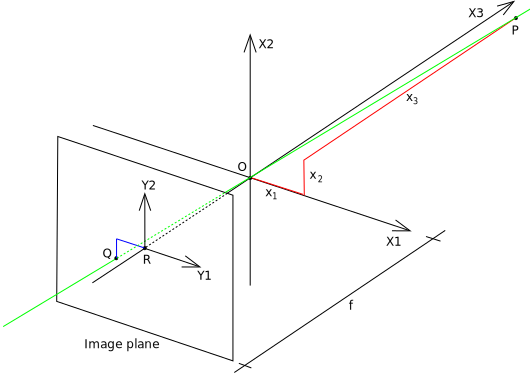
\includegraphics[width=0.7\textwidth]{gfx/pinhole3d}
}{fig:pinhole3d}
{Pinhole camera geometry. Camera coordinate system origin at O, axis X3 points towards the optical axis, Y1 and Y2 point to image plane axes and R is the principal point, at the image center. The point P projects to Q, as well as everything else on the line joining them. The image plane is f units away from camera origin; f is called the focal length.}

In computer graphics and vision, points and directions are usually described in homogeneous coordinates.
Translation, perspective projection, rotation, and other operations are conveniently described as matrices by using an additional dimension for points, of which usually the last element is 1: $(x, y, z, 1)$.
All points $(xw, yw, zw, w)$ map to the same point $(x, y, z)$.
\cite{dubrofsky2009homography,hartley03multiview}

%Homography definition (mapping of points and lines in $P^2$)

The imaging process essentially captures a projection to a flat two-dimensional plane of the camera's view, as described in section \ref{sec:imaging}.
When relating points between different cameras that view the same scene, the cameras' relational positions and rotations must be known.
One of the cameras is often conveniently chosen as the origin of a global coordinate frame, so that its extrinsic parameters become unity transforms (programming libraries often assume this, see e.g. \cite{opencv}).
Each three-dimensional point in the world is transformed to the small sensor or film inside the camera, which is then digitized to a discrete two-dimensional grid of pixels. The size of this pixel array (i.e. image) is referred to as the camera's resolution.

%Figure \ref{fig:TODO} illustrates this transformation chain, which is encoded as the following equations, given a homogeneous point (4-dimensional vector) $X$ representing a 3D location described in physical (e.g. metric) coordinates:

The transformation chain is encoded as follows, given a homogeneous point (4-dimensional vector) $X$ representing a 3D location described in physical (e.g. metric) coordinates:

\begin{align}
	x &= P X\\
	  &= M_i X_s\\ % X_s on the sensor
	  &= M T R X\\
	  &= M_i M_p T R X\\ % R, T camera pose, M_4 to camera sensor, M_3 to pixel coords
\end{align}

$x$ is a 2d pixel in a discrete image, $X_s$ exists on the sensor. $R$, $T$ encode the camera rotation and translation (extrinsics); $M_p$ projects the world coordinates to the camera sensor (film) - still in world coordinates (intrinsics!), and finally the affine $M_i$ transforms the points from the sensor to pixel coordinates on the digital discretized image.

The whole projection $P = M_i M_p T R$ can be used as-is without decomposing it to separate matrices, unless the individual parameters are needed. As the chain consists of several matrices, some of them are defined only up to scale; the coordinate systems' units can be chosen freely. Software packages usually do not decompose the chain, because it is not needed and unique parameters cannot be found because of scaling.

%The external camera parameters are called the extrinsics: camera coordinate system position and rotation (heading) in the global space.
%Camera position sits at the projection center blah.

The internal parameters, intrinsics, encode how the image is formed on the sensor: they consist of focal length, sensor size and principal point: (last column left out, as it's full of zeroes in 3x4)

\begin{equation}
	M =
	\begin{pmatrix}
		m_x & \gamma & u_0\\
		0   &    m_y & v_0\\
		0   &        0 & 1
	\end{pmatrix}
\cdot
	\begin{pmatrix}
		f & 0 & 0\\
		0 & f & 0\\
		0 & 0 & 1
	\end{pmatrix}
	=
	\begin{pmatrix}
		\alpha_x & \gamma   & u_0\\
		0        & \alpha_y & v_0\\
		0        & 0        & 1
	\end{pmatrix}
\end{equation}

For simplicity, it is often denoted $\alpha_x = m_x f$, $\alpha_y = m_y f$. $R = (u_0, v_0)$ is the image center (or principal point). For square pixels, $m_x = m_y$, and for a non-skewed sensor, $\gamma = 0$, which is often the case. \cite{hartley03multiview,szeliski10vision,heyden2005multiple}

%Le image. Horizontal planar triangle, lines between camera origins etc. lecture11.pdf.

% }}} coord systems and transforms

\subsection{Camera calibration} % {{{

Calibration is often specified with a camera projection matrix, or several separate matrices.
It may be convenient to store intrinsics and extrinsics separately if the intrinsic matrix is constant for several pictures, for example (?).

calibration can be automatically determined, given by X corresponding points that can be distinguished in each image and matched [?]. Commonly the points are particular \emph{features}, commonly very noticiable edges or corners, found with an algorithm such as SIFT [?], SURF [?] or Harris corner detector [?]. % feature correspondences

TODO Figure: show extrinsic in matlab cam calibs, nice pics (both cam and world centered)


%In order to accurately measure a scene with a camera, the camera's properties must be known.
Reconstruction algorithms need to relate points between images; the camera properties are needed.
Calibrating a camera means to measure its intrinsics and extrinsics in order to map its data to a known coordinate frame.
Calibration has always to be done, but it does not necessary need to be a manual step before scanning; self-calibration attempts to target this convenience problem. \cite{pollefeys1999hand,hartley03multiview}

%Projective calibration only is too general, as it leaves out some assumptions that can be done about a physical world, such as relative angles and sizes; metric calibration something something. \cite{zisserman1995metric}.

Automatic calibration tools rely on an amount of feature pairs of which the best matches are found, or a known pattern, such as a planar checkerboard pattern \cite{chuang2002performance,zhang2000flexible} whose features are also distinguished with a similar algorithm but a priori knowledge of the object structure is used for precise calibration.
These usually need several pictures taken with the same camera from different poses.

The checkerboard calibration step can also measure optical distortion at the same time. \cite{opencv,camcalmatlab}

%TODO Figure: show extrinsic in matlab cam calibs, nice pics (both cam and world centered)

%Single three-dimensional calibration object is also sufficient blbl

One possible way is direct linear transform (DLT)
\cite{hartley03multiview}: the whole matrix $P$ is solved from $x_i = PX_i$ by constructing a system of equations from the projections of some known points $i$, and minimizing an error metric, as the case is usually overconditioned.

%Methods that dig the matrix out of a single image have certain restrictions, and won't work if e.g. seven points lie on the same plane [longuet-higgins etc.]

%XXX see below. Intrinsic, extrinsic. Distortions. Projection matrices. Camera resectioning.

%many single planar chessboard pics vs. a single image of an accurate 3d model.
%chessboards easier to manufacture at a high precision, just print out and stick to flat surface
%cv::stereocalibrate, cv::calibratecamera
%Single three-dimensional calibration object is also sufficient blbl


%The scale of values in the equations above affects the precision [hartley, in defense of .., h,ziss]. A similarity transform can be used to modify the values to a more consistent range; this is called normalization of the data.

%XXX see below. Intrinsic, extrinsic. Distortions. Projection matrices. Camera resectioning.


% }}} camera calibration

\subsection{Preprocessing/normalization} % {{{

The scale of values in the equations above affects the precision \cite{hartley1997defense,hartley03multiview}.
A similarity transform can be used to modify the values to a more consistent range.

Translate centroid to the origin, scale so that average becomes sqrt 2.

maybe move this to a paragraph as part of another section.

- sync shit

- histogram equalization

- brightness equalization between images

% }}}

\subsection{Calibrated stereo vision} % {{{
% }}}

\subsubsection{Binocular disparity} % {{{

%Essential, fundamental matrices. Correspondence problem. Rectification, undistortion. Epipolar geometry.

\simplefig{h!}{
\begin{tikzpicture}[scale=0.3]
	% P, Z
	\draw[fill] (0, 20) circle [radius=0.3];
	\node at (0, 21) {$P$};

	\draw [<->] (0, 0.5) -- (0, 19.5);
	\node at (0.5, 10) {$Z$};

	% origins, T
	% TODO: circles, node ends not exactly at those points
	\draw [<->] (-9.5,0) -- (9.5, 0);
	\draw[fill] (-10, 0) circle [radius=0.3];
	\draw[fill] ( 10, 0) circle [radius=0.3];
	\node at (-10, -1) {$O_l$};
	\node at (10, -1) {$O_r$};
	\node at (0, -1) {$T$};

	% headings
	\draw [->] (-10, 0) -- (-10, 10);
	\draw [->] (10, 0) -- (10, 10);

	% image planes, at y=4
	\draw[thick] (-13, 4) -- (-7, 4);
	\draw[thick] (13, 4) -- (7, 4);

	\draw [<->] (-6, 0.5) -- (-6, 3.5);
	\node at (-5.5, 2) {$f$};


	% intersection points at principals and xs
	\draw[fill] (-10, 4) circle [radius=0.3];
	\draw[fill] (10, 4) circle [radius=0.3];

	\node at (-10.5, 3) {$c_l$};
	\node at (10.5, 3) {$c_r$};

	\node at (-9, 5) {$x_l$};
	\node at (9, 5) {$x_r$};


	% O-to-P
	\draw (-10, 0) -- (0, 20);
	\draw (10, 0) -- (0, 20);


	% p
	\draw[fill] (8, 4) circle [radius=0.3];
	\node at (8, 3) {$p_r$};
	\draw[fill] (-8, 4) circle [radius=0.3];
	\node at (-8, 3) {$p_l$};
\end{tikzpicture}
}{fig:simplestereo}
{A very simple stereo setup, picture from above. The image planes (thick lines) are actually imaginary, as a real film in a camera would exist behind the principal point and project the image upside down, as described earlier in \ref{sec:imaging}. The coordinates exist in the world coordinate units. The symbols $O$ are the camera origins ($T$ units between each other); $c$ the principal points; $x$ the image plane coordinates of $p$ w.r.t. the principal points; and $f$ is the focal length. The unknown is $Z$, depth of point $P$.}
% this figure would need to be bigger and have also the back side planes (sensors) as opposed to the (normalized?) image planes (at f=1?)

%Next, the setup of binocular stereo vision is described. Common stereo vision rigs use the simplest possible case: two identical cameras with a fixed distance, both oriented to the same direction, parallel to the line connecting them, as in figure \ref{fig:simplestereo}.

Assuming known calibration with identical cameras (same focal length and sensor) in a setup described above, visualized in figure \ref{fig:simplestereo}, points can be triangulated as follows:

From similar triangles with a common vertex at $P$, we get (note that $x_r < 0$ as it's to the left, towards to the negative axis, from the corresponding plane's origin)

\begin{align}
	\frac{Z}{T} &= \frac{Z-f}{T - x_l + x_r} \\
	&= \frac{Z-f}{T - d}\\
	ZT - Zd &= ZT - fT\\
	Z &= \frac{fT}{d} \label{eq:z}
\end{align}

The disparity $d$ is the difference of the points in their image planes, $d = x_r - x_l$.
If the image planes would be fixed as being physically correct, in the back side of the camera origins, the focal length should be negated to keep the correct interpretation and sign because the projected physical image is mirrored in both axes. Image processing between the sensor and a picture file usually inverts this.

As the equation \ref{eq:z} shows, depth is directly inversely proportional to disparity in this simple case.
To map the depth to correct units, only focal length $f$ and the baseline $T$ are needed additionally; when using pixel coordinates instead of physical in $d$, also the pixel size should be taken into account.
All of these are encoded in the camera parameters.
Algorithms such as those in OpenCV \cite{opencv} can compute point clouds from disparity images.

% }}} binocular disparity

\subsubsection{Epipolar geometry} % {{{

\simplefig{h!}{
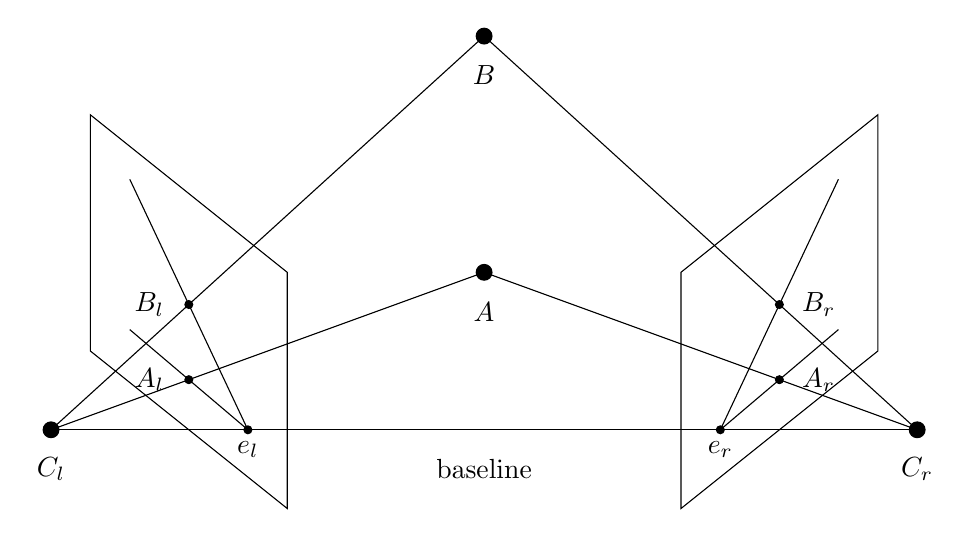
\begin{tikzpicture}[scale=0.5]
	% cameras
	\draw[fill] (-11,-1) circle [radius=0.2];
	\draw[fill] ( 11,-1) circle [radius=0.2];
	\draw (-11,-1) -- (11, -1);
	\node at (0, -2) { baseline };

	\node at (-11,-2) {$C_l$};
	\node at ( 11,-2) {$C_r$};

	% planes
	\draw (-10,1) -- (-10,7) -- (-5,3) -- (-5,-3) -- cycle;
	\draw ( 10,1) -- ( 10,7) -- ( 5,3) -- ( 5,-3) -- cycle;

	% 3d pts
	\draw[fill] ( 0,3) circle [radius=0.2];
	\draw[fill] ( 0,9) circle [radius=0.2];
	\node at (0,2) {$A$};
	\node at (0,8) {$B$};

	% origins via pts
	\draw (-11,-1) -- (0,3) -- (11,-1);
	\draw (-11,-1) -- (0,9) -- (11,-1);

	% epis
	\draw[fill] (-6,-1) circle [radius=0.1];
	\draw[fill] (6,-1) circle [radius=0.1];
	\node at (-6,-1.5) { $e_l$ };
	\node at (6,-1.5) { $e_r$ };

	% projections
	\draw[fill] (-7.5,0.2727) circle [radius=0.1];
	\draw[fill] (-7.5,2.1818) circle [radius=0.1];
	\node at (-8.5, 0.2727) {$A_l$};
	\node at (-8.5, 2.1818) {$B_l$};
	% lines from epis
	\draw (-6,-1) -- +(-2*1.5,2*1.2727);%(-7.5,0.2727);
	\draw (-6,-1) -- +(-2*1.5,2*3.1818);%(-7.5,2.1818);

	\draw[fill] (7.5,0.2727) circle [radius=0.1];
	\draw[fill] (7.5,2.1818) circle [radius=0.1];
	\node at (8.5, 0.2727) {$A_r$};
	\node at (8.5, 2.1818) {$B_r$};
	\draw (6,-1) -- +(2*1.5,2*1.2727);%(7.5,0.2727);
	\draw (6,-1) -- +(2*1.5,2*3.1818);%(7.5,2.1818);
\end{tikzpicture}
}{fig:epigeom}
{Two camera views on same scene.
World points $A$, $B$ project to planes of different views imaged from $C_l$ and $C_r$ on the left ($A_l$ and $B_l$), and to the right ($A_r$, $B_r$).
The actual images cover some area of the total projection plane, and the epipolar point may or may not lie visible in the image.
When $A_l$ is known, its corresponding point $A_r$ (not initially known in practice) is found on the epipolar line joining $e_r$ and $A_r$ in the right image.
All epipolar lines in a view join in the same point ($e_l$ and $e_r$).}
% XXX do i want the planes in physical positions too or another pic to visualize it?

% TODO: small algorithm for pairwise windowed point matching on the line (hox! and link to point matching section maybe)

% what?
Triangulation or reconstruction of the scene structure given by image pair(s) is usually done on the base of a known relationship between the cameras.
Such relationship, known as calibrating the cameras, can be automatically determined, given by corresponding points that can be distinguished in each image and matched.
\cite{trucco1998introductory,hartley03multiview}

In stereo vision, the same scene of interest is seen by two or more cameras at the same time.
The cameras are rarely aligned perfectly such as in the disparity setup described above, however.
Epipolar geometry encodes the relations between arbitrarily positioned cameras in a standard way so that coordinates of a 3D point seen in several images can be calculated with the same triangulation.

A point seen by camera $C_l$ at 3D point A could be anywhere on the line between $C_l$'s origin and P, because a certain line passing through the principal point always projects to a point.
This line is seen as a single point $A_l$.
From another viewpoint in camera $C_r$, this line equals to some line on B's image plane.
The real point must be on that line.
The inverse applies for any point on $C_r$ and a line on $C_l$.
The lines on the image planes are called epipolar lines.

% FIXME:
Essential matrix defines how the camera poses differ by the something something points seen by both.
When $A_l$, $A_r$ encode the points in figure \ref{fig:epigeom} by the corresponding camera coordinates, and the baseline difference (vector from $C_l$ to $C_r$) is marked as $t$, it holds that $(A_l-C_l) \cdot t \times (A_r-C_r) = 0$, as all the vectors are coplanar; the cross product yields a normal to the plane, which is perpendicular to all the vectors, thus the dot product equals 0.
\cite{hartley03multiview}

Essential matrix is a matrix form of this relation; it includes the relative rotation and translation of the two cameras.

%\begin{align*} \label{eq:essential}
%	%A_r &= R (A_l - t) \\
%	%A_r^T R T A_l &= 0 \\
%	%A_r^T E A_l &= 0
%	A_l \cdot t \times A_r = 0\\
%	A_l \cdot t \times R A_r = 0\\
%	A_l^T T
%\end{align*}

%where $T$ is the cross-product form of $t$ encoded in a matrix form as below. The essential matrix is obtained as $E = R T$.
%
%Le image. lecture11.pdf. O->p dot (O->O' cross O'->p') = 0
%
%Cross product expressed in a skew-symmetric matrix form is
%\begin{equation}
%\vec a \times \vec b =
%\begin{pmatrix}
%	 0   & -a_z &  a_y\\
%	 a_z &  0   & -a_x\\
%	-a_y &  a_x & 0
%\end{pmatrix}
%\begin{pmatrix}
%	b_x\\b_y\\b_z
%\end{pmatrix}
%= \vec c
%\end{equation}

Fundamental matrix relates the corresponding points in stereo images; it has the same meaning as the essential matrix, but it works in the pixel coordinates of the cameras, which are obtained after the projective transform that takes the intrinsics into account.
Inverting the matrix $M_i$ (\ref{sec:coord}) in sensor-to-pixel coordinate transform and using it on pixel coordinates, world coordinates seen by the camera can be obtained. % FIXME equations

%\[
%\hat pAl = M_p A_l\\
%\hat A_r = M_p A_r
%\]
%
%and using it on pixel coordinates, the world coords can be obtained, plugging in to the equation \ref{eq:essential}
%
%\[
%A_r^T E A_l = 0\\
%(M_p^-1 \hat A_r)^T E (M_p^-1 \hat A_l) = 0\\
%\hat A_r^T M_p^-T E M_p^-1 A_l = 0\\
%\hat A_r^T F \hat A_l = 0
%\]
%
%the fundamental matrix
%
%\[
%F = M_p^-T E M_p^-1 = M_p^-T R T M_p^-1
%\]

The fundamental matrix relates the pixels and epipolar lines, and as such it is useful in image processing where the images are described as pixels in a color array (image) and not colored physical coordinates.

%Epipole can be interpreted as the location of another camera as seen by other camera.

A point seen by camera A at 3d point P could be anywhere on the line between A's origin and P.
This line is seen as a single point.
From another viewpoint in camera B, this line equals to some line on B's image plane.
The real point must be on that line.
The inverse applies for any point on B and a line on A.
The lines on the image planes are called epipolar lines.

Essential matrix defines how the camera poses differ by the something something points seen by both. $p_l$, $p_r$ 3d points; vectors from camera origins (camera coordinates!) to the same point

\[
	p_l^T E p_l = 0
\]

Le image above and lecture11.pdf. O->p dot (O->O' cross O'->p') = 0

Cross product expressed in a skew-symmetric matrix form is
\begin{equation}
\vec a \times \vec b =
\begin{pmatrix}
	 0   & -a_z &  a_y\\
	 a_z &  0   & -a_x\\
	-a_y &  a_x & 0
\end{pmatrix}
\begin{pmatrix}
	b_x\\b_y\\b_z
\end{pmatrix}
= \vec c
\end{equation}

Fundamental matrix relates the corresponding points in stereo images.

Epipole can be interpreted as the location of another camera as seen by other camera, as seen in the picture.

% }}} epipolar geometry

\subsubsection{Features and point matching} % {{{

salient geometric features for matching

Previously, basics for reconstructing three-dimensional location for a point pair were introduced, assuming known positions for the same point in different images.
To reconstruct a whole scene from a full image, all pairwise points must be matched, i.e. found that what pixel in one view represents the same object as one in other view.

Matching is often also called correspondence searching:
Given a pixel in one image, what is the corresponding pixel in another image taken from the same scene?
Pixels correspond to each other if they represent the same physical point.

% FIXME: pairwise feature matching vs. windowed matching
% TODO some sift descriptor theory, angle histogram stuff

To describe the pixel's characteristics, its surrounding environment is encoded as a \textit{feature}, a easily recognizable, unique property vector.
When discussing about features, not every pixel's neighbourhoods are used; \textit{good} features are those that have strongly distinguishable properties, such as edges and corners.

Edges or corners are essentially high-frequency information in the image that can be interpreted as a 2D discrete function; thus, they can be detected by a discrete high-pass or band-pass filter, zeroing all but those pixels where a high difference is found \cite{marr1980theory}

Neighbourhood of a pixel where features are detected is often called a window or a patch.

% this is kind of the pairwise-vs-windowed stuff
Matching can be done in sparse or dense mode; sparse matching finds a set of features from each image, and tries to match them. Dense matching runs through each pixel of one image and tries to find the same from another one with e.g. template matching \cite{duda1973pattern}; from the coordinate differences in image space between the two images, a disparity map is built. The disparities are then directly transformed to depth values, yielding a point cloud.

Scale-invariant feature transform (SIFT) \cite{lowe1999object} is a commonly used algorithm for local feature detection. A GPU implementation is also available \cite{changchang2007siftgpu}.  Invariance to scaling, translation and rotation makes SIFT useful in describing features that can be matched between unaligned images. Other similar commonly used means are Speede Up Robust Features (SURF) \cite{bay2006surf} Harris corner detector \cite{harris1988combined}.

While SIFT being probably the most popular, other corner detectors are also used, such as Harris and difference-of-gaussian-based (DoG) methods.


% }}}

\subsubsection{Correspondence and rectification} % {{{

% rectification pics

In order to triangulate a real point from two or more photographs, the location of the point in all images must be known.
Rectification is a process that simplifies this search problem by restricting the search to a single dimension.
By aligning the cameras such that their images are coplanar, the search only has to be performed on a line that is parallel to the line connecting the camera centers.
After rectification, the corresponding lines are axis-aligned (horizontal or vertical) in both images. \cite{hartley03multiview}

Rectified images are twisted so that todo todo, see figure \ref{fig:rectification} compare to epipolar geometry image, epipolar lines become parallel in the rectified images
% LOL TODO guido gerig image rectification (stereo) slides

% }}} correspondence and rectification

\subsubsection{Multi-view stereo} % {{{
% (or n-view?)

The case of more cameras than a single pair uses the same principles in epipolar geometry.
It brings more restrictions and dimensions; in three dimensions, for example, the fundamental matrix becomes three-dimensional, the trifocal tensor. \cite{hartley03multiview}
It is also more computationally heavy, as more data must be processed; if no information about camera parameters is available, pairwise checks between the images may become expensive. \cite{wu2013towards}

Multiple baseline stereo is a simple special case for many cameras. When all the cameras lie on the same baseline, calibration is easier and points can be selected by using a minimized sum of errors. \cite{okutomi1993multiple}

The cameras that are used in capturing a scene can be fixed or positioned arbitrarily; in fact, the structure from motion technique \cite{snavely2006photo,fitzgibbon1998automatic} enables to use just one camera that is moved around.
Accurate and fast reconstructions are still traditionally done with stereo camera pairs, though.

Another common way is to use pairwise cameras for individual reconstructions to build a point cloud for every pair, and then register them together. \cite{bradley2010high}

Some suggest to find a set of initial features and expand them to nearby pixels (accuratedense, regiongrowing)

% }}} multi-view stereo

\subsection{Structure from motion} % {{{

The structure from motion (SfM) problem, also called structure and motion, uses the scene feature matches between different views to determine both the scene structure and the camera motion between the views.
The camera does not have to physically move; the method is often used for a multi-camera reconstruction with a static rig.
Before SfM, the images should have been rectified and features matched; the algorithm works on point locations instead of input images.

SfM begins with two reference views that are used to retrieve an initial reconstruction, and extends each new view into the set iteratively.
Lastly, a bundle adjustment method is used to globally optimize the scene parameters.
The relation between the views need not be previously calibrated; the process determines camera poses.
In fact, many reconstruction applications use structure from motion as an initial step with bundle adjustment to determine calibration and proceeds to dense reconstruction.

The initial stage builds a reference frame and structure for the selected features (points).
% pollefeys tutorial builds the frame using the epipolar geometry, determined as previously in section \ref{sec:epipolar}.
The structure is determined with triangulation as in section \ref{sec:binocular}.
In practice, perfect reconstruction cannot be achieved due to noise, and the points are found by minimizing a reprojection error to the extent of a specified threshold limit.

After a coordinate frame is built as a basis using two views, the next camera views are iteratively added to obtain an initial estimate of the camera poses and the selected scene feature positions.
Scene features can be matched between only last few views if the camera motion is known to be continuous;
the matches can also be done between all possible image pairs, which is feasible if there is lots of overlap.

As a last step, bundle adjustment globally optimizes the bundles of light rays from the scene to all cameras.
Several algorithms and implementations are available, while the basic idea and the underlying problem is the same:
a cost function is used to optimize jointly all camera parameter estimates such that the reprojection errors are minimized through all views.
Pollefeys \cite{tutorial} gives the following formula to minimize:

\begin{equation}
	\text{min}_{P_k, M_i} \sum_k=1^m \sum_i=1^n D(m_{ki}, P_k M_i)^2
\end{equation}

when the goal is to find the projection matrices $P_k$ and the 3D points $M_i$ for all views $k$ and points $i$, where $D(a,b)$ is the Euclidean distance and $m_i$ the known, fixed matching 2D image feature positions for each unknown 3D point $M_i$.


% others?

% }}}

\subsection{Error metrics} % {{{

The quality of the reconstruction is measured by reprojecting the 3D points back to the cameras with the estimated parameters, and calculating the distance between the projected and the matching original point. \cite{hartley03multiview}
%This is of course possible only for calibrated objects; no precise errors can be recovered from an unknown structure.

Talk about noise here.

Bundle adjustment \cite{wu2011multicore} seeks to optimize all camera parameters at once with good performance, at the cost of more computation.

A common way to handle feature errors is Random Sample Consensus (RANSAC). Random subsets of the sample space is iterated, and samples that do not fit well to a model that is constructed of a smaller set are ignored. The iteration that matches most samples is selected. \cite{hartley03multiview}

Compare to algebraic, geometric etc.

Detail calculation (error on surface ~= avg reprojection error?) compute millimeters

Mesoscopic level shape reconstruction

% }}}

\subsection{Surface fitting} % {{{
% }}}

\subsubsection{Data structures} % {{{

Should some of the main terms be defined in the beginning of the whole thesis? Probably...

A \textit{(polygon) mesh}, a data structure often used to describe 3D models, consists generally of \textit{vertices} connected by \textit{edges}, forming \textit{faces} of objects. Often, the models only consist of triangles, but other polygons are possible too.
Usually the objects are closed (or ``watertight'') so that all edges are connected to two vertices.

Polygon meshes have an important property that is called \textit{topology} in the context of this thesis.
It refers to the connectivity information of vertices on a surface, describing neighbours of each point.
A \textit{point cloud} is a loose term to describe a disorganized set of 3D points with no topology information; that is, a cloud consists only of a list of vertices, with possibly some attributes such as color or normal.

Stanford bunny or something here as an example of 3D model, or just a cube?

% http://en.wikipedia.org/wiki/File:Mesh_overview.svg

Point cloud is a natural output format for 3D reconstruction, as each point in the cloud would map to some pixel in a source image.
The images and the depth information of the 3D points are not enough for surface information, which is covered next.

% }}} data structures

\subsubsection{Geometry} % {{{

Assuming that the recovered 3D point cloud represents the surface of an object, the next step of interest is to recover the surface topology from the point cloud.
The point cloud is all geometric information that is available, but the images probably consist of more pixels than the number of points in the point cloud.
To work with the generated model and to render it properly with colors, it is imporant to recover the topology information.

A commonly used method in implemented reconstruction programs (e.g. \cite{meshlab}) is Poisson surface reconstruction \cite{kazhdan2013screened}.

Before fitting a surface on the points, the point data set should be processed either manually or automatically to remove outliers.
The surrounding scene might contain geometry that is not part of the scanned object, which will affect badly the surface fitting algorithm.
Manual work is a simple way to delete the points that are not part of the actual object. Automatic methods include (TODO)

% }}} geometry

\subsubsection{Texture reprojection} % {{{

When a polygon mesh is available, it should be rendered in color. The de facto method in computer graphics is to uses \textit{texture mapping} to color pixels in between the vertices.

use the registered raster projections to find out best textures and build uv coordinates

% }}} textures

\subsection{Postprocessing} % {{{

Talk about how the stored geometry is different from the rendered one; mathematical models in fragment shaders to use the texture variations / normal maps etc.

Error removal; strip outliers that do not have nearby pairs; small disconnected islands.

Postprocessing: remodel the mesh (face), see what it would look like.
Refine parameters to get a similar output as in the photos (normal map etc.), backproject.
Use colors and highpass them; assume uniform lighting and locally uniform texture color (bradley).
(Simply a rendering technique, that level of detail in 3D structure might not be needed).
Still, structured light and/or shading assumptions [shape from single image cues/shading trucco+verri p.225] done too.

(video: 3d topology different in each frame; most algos do just stills. simple to combine them to a pre-recorded mesh)

Rendered facial animation: google up on bones and stuff.
% }}}

\clearpage
\section{Motion capture}

surface vs motion capture

Motion capture seeks to fit a sequence of movements to a model by recording the movement and processing the data to be used with the model. \cite{find-a-definition-somewhere}

% It is possible to assume locally smooth movements in most areas; thus, a more intelligent approach should be used than simply reconstructing a new mesh for each frame and using registration to just align them.
% By making certain assumptions on high-resolution texture, very detailed bump maps can be extracted, for example, by backprojecting the expected 3d mesh to textures and refining. [CITE]


\subsection{4D data capture} % {{{

The industry uses the term 4D in the context of time-varying 3D data.

A naive registration to e.g. previous or first frame is possible to average out the object movement if only its local surface movement is of interest.
Still, this will not produce the same topology for the mesh, as each frame contains different point cloud and is not connected to the previous reconstruction, unless some algorithm that takes this into account is used.

One possible method to correct the lack of geometric structure is to fit each frame of the mesh to another pre-recorded or pre-modeled mesh. \cite{somewhere,remedysoftware?}
This can be beneficial because the raw reconstruction quality may be even too high for practical use.

Later usage may need only the tracked positions of specific locations on the surface to deform a mesh in some custom way.

% }}}

\subsection{Tracking the geometry} % {{{

Kalman

Fiducials / AR

perf of cloth anim capture

Analogous to the case of traditional 2D video consisting of separate discrete frames of pixels, a dynamic stream of 3D data is, in a simple case, individual ``frames'' of point sets.

The dynamic case requires tracking of individual points or objects in order to usefully handle the moved object(s).
Non-static human motion capture cases in video gaming or movies where post-processing time is available rely on manual work to perfect the quality.
A realtime case would need to e.g.~automatically register each frame between the previous one to use the geometry's dynamic properties.

The simplest tracking step is to leave tracking out completely: depending on the application, tracking might not be needed if the work done on the three-dimensional data does not need e.g. topological continuity in the time domain, but recomputes its work on each new point cloud.

Registration and tracking of point clouds or meshes is a large topic on its own; this section reviewes only some of the most common methods presented in the literature. Some work with the reconstructed 3D structure; others use the source images and do additional work.

Disorganised nature of the result data topology in frame-per-frame capture make it challenging to track individual points.
In three dimensions, a template model is often scanned beforehand that is then morphed to match the target object to keep the topology (i.e.~vertex neighborhood connectivity) constant.
This technique adapts to both static and rigid cases.
\cite{bojsen2012tracking,li2009robust}

Common method also for the entertainment industry is to use a pre-determined model of the scanned target or a completely separate character, and deform it on each frame based on the current state of the object, fitting the model's vertices to the scanned set.

Facial animation does not necessarily even need multi-view stereo for tracking and driving a predesigned character \cite{chuang2002performance,deng2007computer}.

% }}} tracking

\subsection{2D features / surface tracking} % {{{

* SIFT/SURF/Harris feature tracking, reproject

* edgels (edge pixels)

In two dimensions, the full reconstruction step can be skipped when using only features in image space, providing real-time performance. \cite{pilet2005real}
When assuming that a precise object stays in the cameras, features can be detected and tracked locally with no reprojection, while the tracked object is assumed to keep the same topology as a previously scanned model.

Pore-level matching, good resolution needed

Many cameras, zoom in to just a part of the target

Markers / markerless

Markers traditional

%http://en.wikipedia.org/wiki/Facial_motion_capture the polar express, beowulf

This work considers markerless capture important, because time-varying texture is important in facial capture (wrinkles from different facial expressions)

Special marker makeup / pre-recording of pore-level texture? Then "good enough" zillion markers and map and deform the mesh?

Corner detector (harris, sift, surf). Color usually not important. Brightness constancy. Repeated texture or no texture (uniform color = bad).

Matching to a priori model

% }}} 2d features

\subsection{Registration} % {{{

Combining 3D meshes from multiple viewpoints (cameras/camera pairs). Also e.g. ransac for removing noise. Iterative closest point fitting.


When reconstructing an object all over again in consecutive frames, the points might not be fully aligned, and more importantly, they do not share the same model topology, i.e. the vertices have no other relation to the vertices in previous frames than being spatially near each other, accompanied with noise. \cite{zhao2005alignment}

Registration aligns disoriented models (e.g. point clouds, surfaces or triangular meshes, depending on the application) together with a rigid transformation between them so that one becomes the other from a reference coordinate frame's viewpoint.
Aligning two geometrically \textit{same} objects may not hold if the object deforms in a non-rigid way; when tracking the motion/deformation of a surface, the point sets describe a different geometry and there will always be some error.

A common method is Iterative Closest Point (ICP): iterative refinement approach to move the meshes closer to each other a small step at a time.
When ICP is used locally, it can be applied to non-rigid cases too. \cite{brown2007global}

% }}} registration

\subsection{Optical flow} % {{{

Long history; several mature commercial video editing products. The Matrix.

Uses: Frame time offset compensation by interpolation (morphing), needs features, direction vector estimation

Motion in an image shows as changes in pixel color; it can be perceived as similar pixels flowing to the direction of movement in a pattern.
A motion vector can be calculated for each pixel, resulting in a vector field; following and interpolating the movement is another way to detect three-dimensional movement.
\cite{gibson1950perception,horn1981determining,beauchemin1995computation}

By combining the movement tracking to a mesh whose dynamics are modeled physically, motion can be estimated from a single image.
\cite{decarlo1996integration}

% }}} optical flow

\subsection{(Kalman methods)} % {{{

Is such complexity needed?

% }}}

\subsection{Playback interpolation / morphing} % {{{

The record rate might not be exactly the same as the playback rate; when the movement is displayed on a screen, the positions of the tracked parts of object are interpolated between recorded keypoints.
The same stuff in 2D is called morphing: pixel movement is tracked instead of simply blending each pixel between two time points.

Linear, cubic etc. interpolation.

% }}}
